% =====================================================================
%  Unit 3 -- Reliable models
%  (this file is assembled from src/ch03/*.tex by build_chapter.py)
% =====================================================================
\chapter{Reliable Models}\label{ch:reliable}

In January 2021, the government of the Netherlands resigned over a scandal in which the tax authorities had
wrongly accused thousands of families of defrauding the system of childcare benefits, demanding that they repay
large sums and pushing many of them into debt. Among the tools that selected applications for scrutiny was a
risk-classification model that, among other indicators, took into account whether the applicant had Dutch
nationality \citep{amnesty2021xenophobic}. The model may well have been accurate by some measure; it was neither
fair, nor understandable to the people it judged, nor subject to effective human oversight.

A model can be accurate and still be unacceptable. It may treat some groups of people worse
than others, rely on spurious correlations that will not hold tomorrow, be impossible to
understand or audit, or be easy to fool by someone who wants it to fail. This unit studies four
aspects of the \emph{reliability} of models that go beyond the metrics of \cref{ch:evaluation}:
\emph{fairness\index{fairness|textbf}} (are decisions made the right way and for the right reasons?), \emph{causality\index{causality|textbf}}
(what would happen if we acted?), \emph{interpretability\index{interpretability|textbf}} (can we understand why a model
decides what it decides?) and \emph{security} (can the model withstand an adversary?). The four
are closely connected: we need causal reasoning to talk about discrimination, explanations to
detect unfairness and vulnerabilities, and an understanding of attacks to trust explanations. We close with
the European AI Act\index{AI Act}, which turns many of these concerns into legal obligations.

\begin{objectives}
After studying this unit you should be able to:
\begin{itemize}
  \item recognise the sources of unfairness along the life cycle of a data-driven decision
        system (measurement, learning, action and feedback);
  \item define and compute the main group fairness criteria (independence, separation\index{fairness!separation} and
        sufficiency\index{fairness!sufficiency}), explain why they are generally incompatible, and know the techniques that
        enforce them;
  \item reason with structural causal models\index{structural causal model}: distinguish conditioning from intervening,
        identify confounders\index{confounder}, mediators\index{mediator} and colliders\index{collider}, apply the adjustment formula, and compute
        counterfactuals\index{counterfactual};
  \item explain why interpretability matters, classify interpretability methods, and interpret
        linear models, logistic regression\index{logistic regression}, trees and rules;
  \item apply model-agnostic methods (partial dependence\index{partial dependence plot}, ICE\index{individual conditional expectation}, interaction strength,
        permutation importance\index{feature importance!permutation}, surrogates\index{global surrogate}, LIME\index{LIME} and Shapley\index{Shapley values} values) and example-based
        explanations (counterfactuals, prototypes\index{prototypes and criticisms} and criticisms, influential instances\index{influential instance}),
        knowing their limitations;
  \item describe the main attacks on machine learning systems (poisoning\index{poisoning attack}, evasion\index{evasion attack}, transfer)
        and the defensive measures, with their limits.
  \item explain the risk-based approach of the European AI Act, and relate the obligations for high-risk\index{AI Act!high-risk systems}
        systems to the techniques of this book.
\end{itemize}
\end{objectives}

% =====================================================================
\section{Fairness in machine learning}\label{sec:fairness}

\subsection{Why fairness?}

Data-driven decisions promise to be better than decisions based on intuition: they take the
available evidence into account, they can be checked, and machine learning can uncover
relevant factors that people would overlook. But learning from examples is induction, and
induction is only as reliable as its examples: they must be sufficient, diverse and well
annotated. If the examples reflect historical prejudices, a model learned from them will
reproduce those prejudices, often in a way that is harder to see.

Disparities do not require bad intentions. In 2016, an analysis of a same-day delivery service
of a large online retailer found that, in several US cities, the neighbourhoods selected for the
service were disproportionately white \citep{ingold2016amazon}. We do not know how that system
works, nor whether it uses machine learning; but the example shows how a decision that seems
neutral (``offer the service where it is profitable'') can produce stark demographic
differences. Whether a disparity amounts to \emph{discrimination} depends on whether it is
justified and whether it is harmful, questions that rarely have simple answers and on which
philosophy, law and sociology have much to say \citep{barocas2023fairness}.

\subsection{The machine learning loop}

Unfairness can enter at every stage of a system that produces decisions with machine learning
(\cref{fig:mlloop}).

\begin{figure}[htbp]
\centering
\begin{tikzpicture}[font=\small\sffamily,
  st/.style={draw=edmnavy,fill=edmnavy!6,rounded corners=3pt,minimum width=26mm,minimum height=9mm,align=center},
  arr/.style={-{Stealth[length=2.2mm]},edmnavy,thick}]
  \node[st] (w) at (0,0) {world\\(individuals)};
  \node[st] (d) at (5,0) {data};
  \node[st] (m) at (10,0) {model};
  \node[st] (a) at (5,-2.3) {actions\\(decisions)};
  \draw[arr] (w) -- node[above,font=\scriptsize\sffamily] {measurement} (d);
  \draw[arr] (d) -- node[above,font=\scriptsize\sffamily] {learning} (m);
  \draw[arr] (m) |- node[pos=0.25,right,font=\scriptsize\sffamily] {prediction} (a);
  \draw[arr] (a) -| node[pos=0.75,left,font=\scriptsize\sffamily] {impact} (w);
  \draw[arr,dashed,edmcoral] (a) -- node[right,font=\scriptsize\sffamily,text=edmcoral] {feedback} (d);
\end{tikzpicture}
\caption{The stages of a machine learning system that makes decisions about people. Each
arrow is a possible source of unfairness.}
\label{fig:mlloop}
\end{figure}

\paragraph{Measurement} Turning the world into data requires subjective decisions and is full of
technical difficulties. The target variable is often a construct that cannot be measured
directly (``creditworthiness'', ``a good employee'') and is replaced by a measurable proxy\index{proxy variable},
whose biases the model will inherit. A widely used algorithm for allocating extra care to
patients in the United States predicted future health \emph{costs} as a proxy for health
\emph{needs}; because less money had historically been spent on Black patients with the same
needs, the algorithm systematically underestimated their needs \citep{obermeyer2019dissecting}.
Variables recorded by decision makers (who was granted bail, who was arrested) measure their
decisions as much as the underlying phenomenon, and data sets repurposed from another use carry
the choices of their original creators. Knowing the \emph{provenance} of the data is crucial.

\paragraph{Learning} A learning algorithm can preserve, mitigate or exacerbate the disparities in
its data, and it has no general way of telling legitimate patterns from stereotypes. Minority
groups are, by definition, represented by fewer examples, so their patterns are learned less
accurately, and the desire to avoid overfitting\index{overfitting} can make the algorithm treat genuine differences
as noise. A single accuracy\index{accuracy} figure hides these differences: commercial face analysis systems
that were very accurate on average had error rates\index{error rate} many times higher for darker-skinned women
than for lighter-skinned men \citep{buolamwini2018gender}.

\paragraph{Action} A prediction is not a decision. Predicting who will fail a course is
different from deciding what to do about it, and decisions that are fairly rendered under unfair
circumstances may do little to improve people's lives. Moreover, the errors of a model may be
unequally distributed between groups, so that the cost of the mistakes falls on some people more
than on others.

\paragraph{Feedback} Decisions change the world that produces the next data. Predictions can be
\emph{self-fulfilling}: if police are sent where the model predicts crime, more crime is recorded
there, which confirms the prediction \citep{ensign2018runaway}. Recommendations determine which
items users can click, and hence the training data\index{training set} of the next model; and predictions can change
the phenomenon they predict (a route predicted to be fast attracts traffic and stops being fast).
Feedback from users can also carry cultural prejudices, for instance when performance reviews
are used as a target.

\paragraph{Other ethical considerations} Training data must be diverse enough for the
population the system will serve, and systems can perpetuate stereotypes: word embeddings\index{embedding} learned
from text associate occupations with genders in ways that reflect, and can reinforce, social
stereotypes \citep{bolukbasi2016man}.

\begin{keyidea}
There are reasons to be cautiously optimistic: data-driven decision making forces us to
articulate the objectives of a decision, makes the decision process more transparent and
auditable than many human decisions, and allows effective intervention\index{intervention}. But fairness\index{fairness} cannot be
reduced to an algorithmic stamp of approval. The value of the formal tools of this section is
that they make it harder to avoid the difficult questions.
\end{keyidea}

% ---------------------------------------------------------------------
\section{Fairness criteria for classification}\label{sec:fairnesscriteria}

We consider a classification problem with features $X$, a target $Y$ and a \emph{sensitive
attribute\index{protected attribute|textbf}} $A$ (gender, ethnicity, age, religion\dots) that defines the groups whose treatment we
want to compare. The classifier is usually a \emph{score} $R=r(X)$, a single number that
summarises the features, turned into a decision by a threshold\index{threshold} (\cref{sec:roc}).

\subsection{No fairness through unawareness}

The first intuition is to remove $A$ from the features. It does not work. In large feature
spaces sensitive attributes\index{protected attribute} are generally \emph{redundantly encoded}: they can be predicted from
the other features (place of residence, shopping habits, browsing history, even genetic markers),
and a model that does not see $A$ can still treat the groups very differently. Removing the
sensitive attribute can even be harmful, for instance in medicine, where a variable such as sex
or ethnicity may be needed to give everyone an accurate prediction.

\Cref{lst:unawareness} uses the synthetic credit data of \cref{sec:creditcase}. The features
(income, debt and a ``zip code'' that summarises the neighbourhood) predict the group of an
applicant with an AUC\index{area under the ROC curve (AUC)} of 0.967. A logistic regression trained \emph{without} $A$ accepts 41\% of
the applicants of group $a$ and 13\% of those of group $b$, and it gives a negative weight to the
zip code, which acts as a proxy\index{proxy variable} of the group. Removing the zip code changes little (40\% against
16\%), because income and debt also differ between the groups.

\begin{pylisting}[label={lst:unawareness}]{Removing the sensitive attribute does not remove its influence}
import numpy as np
from sklearn.linear_model import LogisticRegression
from sklearn.metrics import roc_auc_score
from sklearn.model_selection import cross_val_predict, train_test_split
from credit import credit_data

# X = (income, debt, zipcode); A is not in X
X, A, Y = credit_data(40000)
pA = cross_val_predict(LogisticRegression(), X, A, cv=5, method="predict_proba")[:, 1]
print(f"AUC of predicting the group from the features: {roc_auc_score(A, pA):.3f}")

X_tr, X_te, A_tr, A_te, Y_tr, Y_te = train_test_split(X, A, Y, test_size=0.5,
                                                      random_state=0)
for cols, name in [([0, 1, 2], "income, debt, zipcode"), ([0, 1], "income, debt")]:
    m = LogisticRegression().fit(X_tr[:, cols], Y_tr)
    accept = m.predict_proba(X_te[:, cols])[:, 1] >= 0.8         # lend if P(repay) >= 0.8
    print(f"{name:21s} weights={np.round(m.coef_[0], 2)}  "
          f"acceptance a={accept[A_te == 0].mean():.2f} b={accept[A_te == 1].mean():.2f}")
print(f"repayment rate: a={Y[A == 0].mean():.2f}  b={Y[A == 1].mean():.2f}")
\end{pylisting}
\begin{pyoutput}
AUC of predicting the group from the features: 0.967
income, debt, zipcode weights=[ 0.49 -0.17 -0.13]  acceptance a=0.41 b=0.13
income, debt          weights=[ 0.5  -0.17]  acceptance a=0.40 b=0.16
repayment rate: a=0.70  b=0.50
\end{pyoutput}

\subsection{Three formal criteria}

Most formal non-discrimination criteria are properties of the joint distribution of the
sensitive attribute\index{protected attribute} $A$, the target $Y$ and the score $R$, and they fall into three groups, each a
(conditional) independence statement \citep{barocas2023fairness} (\cref{tab:faircriteria}).

\begin{table}[htbp]
\centering\small
\caption{The three families of group fairness criteria.}\label{tab:faircriteria}
\begin{tabularx}{\textwidth}{@{}llX@{}}
\toprule
Criterion & Independence & In a binary classifier\\
\midrule
Independence & $R\perp A$ & equal acceptance rates (demographic parity)\\
Separation & $R\perp A\mid Y$ & equal true positive and false positive rates (equalised odds)\\
Sufficiency & $Y\perp A\mid R$ & equal predictive values; calibration by group\\
\bottomrule
\end{tabularx}
\end{table}

\paragraph{Independence} The score must be independent of the sensitive attribute. For a binary
decision this means that the probability of a positive decision is the same in all groups,
$P\{R=1\mid A=a\}=P\{R=1\mid A=b\}$, a criterion known as \emph{demographic} or
\emph{statistical parity\index{fairness!demographic parity|textbf}}. It can be relaxed to a maximum difference,
$P\{R=1\mid A=a\}\geq P\{R=1\mid A=b\}-\epsilon$, or to a ratio: the ``four-fifths rule'' of US
employment law considers a selection rate of a group below 80\% of that of the most favoured group
as evidence of adverse impact \citep{feldman2015certifying}. For scores, independence can be
measured by the mutual information $I(A;R)=H(A)+H(R)-H(A,R)$, which is zero under independence.

Independence has important limitations. It can be satisfied in undesirable ways: a lender could
accept the most solvent applicants of one group and a random selection of the same size of the
other, which equalises the rates while being careless with the second group. And when the target
is genuinely correlated with the group, a perfect classifier violates it. There are three families
of techniques to achieve it (and, adapted, the other criteria): \emph{pre-processing}, which
adjusts the data or the feature space so that it is uncorrelated with the sensitive attribute
(for instance, by reweighting the examples, \citealp{kamiran2012data}); \emph{in-processing},
which adds a fairness\index{fairness} constraint or penalty to the optimisation problem of the learner
\citep{zafar2017fairness,agarwal2018reductions}; and \emph{post-processing}, which adjusts a
learned classifier, typically with group-specific thresholds.

\paragraph{Separation} Often the sensitive attribute is correlated with the target, and part of
the correlation is legitimate. Separation\index{fairness!separation} allows the score to depend on $A$ only through the
target: $R\perp A\mid Y$. For a binary classifier,
\begin{align}
  P\{R=1\mid Y=1,A=a\}&=P\{R=1\mid Y=1,A=b\},\\
  P\{R=1\mid Y=0,A=a\}&=P\{R=1\mid Y=0,A=b\},
\end{align}
that is, equal true positive rates\index{true positive rate} and equal false positive rates\index{false positive rate} in all groups
(\emph{equalised odds\index{fairness!equalised odds|textbf}}): the errors of the classifier are equally distributed. A common
relaxation requires only one of the two equalities, for instance equal true positive rates
(\emph{equality of opportunity\index{fairness!equal opportunity|textbf}}, \citealp{hardt2016equality}). Separation can be achieved by
post-processing without retraining, using the ROC curves\index{ROC curve} of \cref{sec:roc}: each group has its
own ROC curve, and the achievable operating points\index{operating point} that satisfy separation are those in the
intersection of the regions under the group curves; the decision maker picks the cheapest one,
possibly randomising between two thresholds \citep{hardt2016equality}.

\paragraph{Sufficiency} The score must capture everything that the group says about the target,
$Y\perp A\mid R$: once the score is known, the group adds no information,
\begin{equation}
  P\{Y=1\mid R=r,A=a\}=P\{Y=1\mid R=r,A=b\}.
\end{equation}
For a binary classifier this means equal positive and negative predictive values\index{predictive value!negative} in all groups.
For a probabilistic score it is closely related to \emph{calibration\index{calibration|textbf} by group},
$P\{Y=1\mid R=r,A=a\}=r$ for all groups $a$ (\cref{sec:calibration}). An unconstrained model that fits the data
well often comes close to calibration in the groups it can identify, but this depends on the learner,
its capacity, the information available and the data, and it must be checked.

\Cref{lst:fairmetrics} computes the three criteria for the credit model with the profit-optimal
threshold of 0.8. In both groups the mean score equals the repayment rate within 0.002, which checks calibration
only on average; the reliability curves of \cref{fig:fairnesscredit}c stay close to the diagonal across
score levels, so the \emph{score} is approximately calibrated by group. The \emph{decision} is another
matter: its positive predictive values\index{predictive value!positive} are similar (0.90 and 0.86), but its negative predictive values
are not (0.44 and 0.55), so the thresholded decision does not satisfy sufficiency\index{fairness!sufficiency}: thresholding a
calibrated score need not preserve it. Independence is far from holding: the acceptance rate of group $b$ is 32\% of that of
group $a$, well below four fifths. Separation does not hold either: the true positive rate, the
fraction of applicants who would repay that get a loan, is 0.53 in group $a$ and only 0.23 in
group $b$.

\begin{pylisting}[label={lst:fairmetrics}]{Independence, separation and sufficiency of a credit score}
import numpy as np
from sklearn.linear_model import LogisticRegression
from sklearn.model_selection import train_test_split
from credit import credit_data

X, A, Y = credit_data(40000)
X_tr, X_te, A_tr, A_te, Y_tr, Y_te = train_test_split(X, A, Y, test_size=0.5,
                                                      random_state=0)
R = LogisticRegression().fit(X_tr, Y_tr).predict_proba(X_te)[:, 1]   # score (A not used)
D = R >= 0.8                                                          # decision: lend
for g, name in [(0, "a"), (1, "b")]:
    m = A_te == g
    gap = R[m].mean() - Y_te[m].mean()  # calibration-in-the-large
    print(f"group {name}: base={Y_te[m].mean():.2f} accept={D[m].mean():.2f} "
          f"TPR={D[m & (Y_te == 1)].mean():.2f} FPR={D[m & (Y_te == 0)].mean():.2f} "
          f"score-base={gap:+.3f}")
    print(f"         PPV={Y_te[m & D].mean():.2f} NPV={1 - Y_te[m & ~D].mean():.2f}"
          f"  (predictive values of the decision)")
print(f"demographic parity ratio b/a = {D[A_te == 1].mean() / D[A_te == 0].mean():.2f}")
\end{pylisting}
\begin{pyoutput}
group a: base=0.70 accept=0.41 TPR=0.53 FPR=0.14 score-base=-0.002
         PPV=0.90 NPV=0.44  (predictive values of the decision)
group b: base=0.50 accept=0.13 TPR=0.23 FPR=0.04 score-base=-0.001
         PPV=0.86 NPV=0.55  (predictive values of the decision)
demographic parity ratio b/a = 0.32
\end{pyoutput}

\subsection{The criteria are incompatible}

These criteria cannot, in general, be satisfied simultaneously \citep{kleinberg2017inherent,chouldechova2017fair}:
\begin{itemize}
  \item independence and sufficiency\index{fairness!sufficiency} are mutually exclusive when $A$ and $Y$ are not independent;
  \item independence and separation\index{fairness!separation} are mutually exclusive when $A$ and $Y$ are not independent
        and the score is informative ($R$ is not independent of $Y$);
  \item separation and sufficiency together lead to degenerate solutions unless the groups have
        the same base rates or the classifier is perfect.
\end{itemize}
The last incompatibility follows from an identity that relates the error rates\index{error rate} of a binary
classifier in a group with prevalence\index{prevalence} $p=P\{Y=1\}$ \citep{chouldechova2017fair}:
\begin{equation}\label{eq:chouldechova}
  \FPR=\frac{p}{1-p}\cdot\frac{1-\PPV}{\PPV}\cdot\TPR .
\end{equation}
If two groups have different prevalences, equal predictive values (sufficiency) and equal true
positive rates\index{true positive rate} force different false positive rates\index{false positive rate}. In \cref{lst:fairmetrics}, group $a$ has
$p=0.70$, $\PPV=0.90$ and $\TPR=0.53$, which gives $\FPR=\frac{0.7}{0.3}\cdot\frac{0.1}{0.9}\cdot0.53
\approx0.14$, while group $b$, with $p=0.50$, has $\FPR\approx0.04$. Choosing a criterion is
therefore a choice about which errors, and whose, matter most.

\subsection{The limits of observational criteria}

All the criteria above are \emph{observational}: they depend only on the joint distribution of
$(A,Y,R)$ and the features. Two scenarios with very different mechanisms can produce exactly the
same distribution. Imagine a model that predicts whether someone is a software engineer. In one
scenario, its features are visits to a website popular among one gender and to a code-hosting
platform; in the other, whether the person studied computer science and attended a conference for
women in computing. Both kinds of features can be correlated with gender in the same way, so any
observational criterion gives the same verdict in both cases, although we may judge them very
differently. Observational criteria cannot tell us whether a classifier uses the sensitive
attribute\index{protected attribute}, nor evaluate alternatives to the data we have. To go further we need to reason about
how the data were generated: measurement and causality\index{causality} (\cref{sec:causality}).

\begin{pitfall}
A fairness\index{fairness} criterion is a diagnostic, not a certificate. We cannot base a conclusive argument
of fairness or unfairness on the value of a single observational criterion; and the criteria can
be manipulated by changing the real-world processes that the data reflect, sometimes in harmful
ways.
\end{pitfall}

% ---------------------------------------------------------------------
\section{Case study: credit scoring}\label{sec:creditcase}

A bank decides whether to grant a loan to each applicant based on a score $R$, the predicted
probability of repayment. A repaid loan earns 1 unit and a default costs 4 units, so the
profit-maximising decision is to lend when $R\geq0.8$ (\cref{sec:costs}). The applicants belong to
two groups: group $b$, 30\% of the population, has a lower average creditworthiness for
historical reasons, and its repayment rate is 50\% against 70\% in group $a$. The data are
synthetic (\cref{lst:credit}), which lets us know exactly how they were generated.

\begin{pylisting}[label={lst:credit}]{Synthetic credit data and four lending policies}
"""Synthetic credit-scoring data and four lending policies (Unit 3)."""
import numpy as np

def credit_data(n, seed=0):
    """Two groups of applicants; group b (A=1, 30%) is less creditworthy on average."""
    rng = np.random.default_rng(seed)
    A = (rng.random(n) < 0.3).astype(int)
    z = rng.normal(0, 1, n) - 0.8 * A                       # latent creditworthiness
    Y = (rng.random(n) < 1 / (1 + np.exp(-(1.5 * z + 1.2)))).astype(int)   # 1 = repays
    income = 2.0 * z + rng.normal(0, 1, n)
    debt = -1.0 * z + rng.normal(0, 1.2, n)
    zipcode = 1.5 * A + rng.normal(0, 0.6, n)               # neighbourhood: a proxy of A
    return np.c_[income, debt, zipcode], A, Y

GAIN, LOSS = 1.0, 4.0                    # profit of a repaid loan, loss of a default

def profit(R, A, Y, t):
    """Profit of accepting the applicants whose score reaches their group's threshold."""
    accept = R >= np.asarray(t)[A]
    return GAIN * np.sum(accept & (Y == 1)) - LOSS * np.sum(accept & (Y == 0))

def four_policies(R, A, Y):
    """Thresholds (group a, group b) of four lending policies, each maximising profit."""
    grid = np.quantile(R, np.linspace(0, 1, 401))           # candidate thresholds
    rates = np.linspace(0.005, 0.995, 199)                  # candidate common rates
    best = lambda cands: max(cands, key=lambda t: profit(R, A, Y, t))
    # threshold accepting a fraction r
    q = lambda mask, r: np.quantile(R[mask], 1 - r)

    # best threshold within one group
    def group_best(g):
        m = A == g
        return max(grid, key=lambda s: profit(R[m], np.zeros(m.sum(), int), Y[m], (s,)))

    return {"max profit": (group_best(0), group_best(1)),
            "single threshold": best([(s, s) for s in grid]),
            "independence": best([(q(A == 0, r), q(A == 1, r)) for r in rates]),
            "equal opportunity": best([(q((A == 0) & (Y == 1), r),
                                       q((A == 1) & (Y == 1), r)) for r in rates])}
\end{pylisting}

The bank compares four lending policies, each maximising profit subject to a different
constraint, by choosing one threshold per group \citep{barocas2023fairness}:
\begin{itemize}
  \item \emph{maximum profit}: possibly different thresholds for each group, chosen only to
        maximise profit;
  \item \emph{single threshold\index{threshold|textbf}}: the same threshold for all the groups;
  \item \emph{independence}: equal acceptance rates in all the groups;
  \item \emph{equality of opportunity\index{fairness!equal opportunity|textbf}}: equal true positive rates\index{true positive rate} in all the groups. It is half of
        separation\index{fairness!separation}, which also requires equal false positive rates\index{false positive rate} (equalized odds\index{fairness!equalised odds}).
\end{itemize}

\begin{pylisting}[label={lst:policies}]{Thresholds, rates and profit of the four lending policies}
import numpy as np
from sklearn.linear_model import LogisticRegression
from sklearn.model_selection import train_test_split
from credit import credit_data, four_policies, profit

X, A, Y = credit_data(40000)
X_tr, X_te, A_tr, A_te, Y_tr, Y_te = train_test_split(X, A, Y, test_size=0.5,
                                                      random_state=0)
X_va, X_te, A_va, A_te, Y_va, Y_te = train_test_split(X_te, A_te, Y_te, test_size=0.5,
                                                      random_state=1)
model = LogisticRegression().fit(X_tr, Y_tr)
R_va, R = model.predict_proba(X_va)[:, 1], model.predict_proba(X_te)[:, 1]
policies = four_policies(R_va, A_va, Y_va)       # thresholds chosen on validation
# ... and evaluated, held fixed, on the test data
top = profit(R, A_te, Y_te, policies["max profit"])
print("test data         thresholds  acceptance    TPR         FPR      profit")
for name, t in policies.items():
    acc = R >= np.asarray(t)[A_te]
    rate = lambda m: f"{acc[m & (A_te == 0)].mean():.2f} {acc[m & (A_te == 1)].mean():.2f}"
    print(f"{name:17s} {t[0]:.2f} {t[1]:.2f}   {rate(Y_te >= 0)}    {rate(Y_te == 1)}   "
          f"{rate(Y_te == 0)}   {profit(R, A_te, Y_te, t) / top:.1%}")
\end{pylisting}
\begin{pyoutput}
test data         thresholds  acceptance    TPR         FPR      profit
max profit        0.80 0.79   0.41 0.15    0.53 0.25   0.15 0.05   100.0%
single threshold  0.80 0.80   0.41 0.14    0.53 0.24   0.15 0.04   99.6%
independence      0.86 0.67   0.27 0.31    0.36 0.48   0.07 0.13   78.6%
equal opportunity 0.84 0.67   0.33 0.30    0.42 0.47   0.10 0.13   81.6%
\end{pyoutput}

The thresholds are chosen on validation data\index{validation set} and then held fixed on a separate test set\index{test set}, whose
results \cref{lst:policies} and \cref{fig:fairnesscredit} show. Because the score is calibrated in
both groups, the maximum-profit thresholds are practically the same (0.80 and 0.79) and the single
threshold loses only 0.4\% of the profit; both accept 41\% of group $a$ and 14--15\% of group $b$.
Independence, which equalised the acceptance rates on the validation data, raises the threshold of
group $a$ to 0.86 and lowers that of group $b$ to 0.67. On the test data the acceptance rates are 27\%
and 31\%, close but not equal, as must be expected on new data; the policy costs 21\% of the profit,
and group $b$ now receives loans that are more likely to default (its false positive rate rises from
0.04 to 0.13). Equality of opportunity gives true positive rates of 0.42 and 0.47 on the test data and
costs 18\% of the profit. It constrains only the true positive rates: full separation would also
equalise the false positive rates (0.10 and 0.13 here), which may require randomised decisions
\citep{hardt2016equality}. In a real bank, moreover, repayment is observed only for the loans that
were granted, while the simulation knows the outcome of every applicant.

\begin{figure}[htbp]
\centering
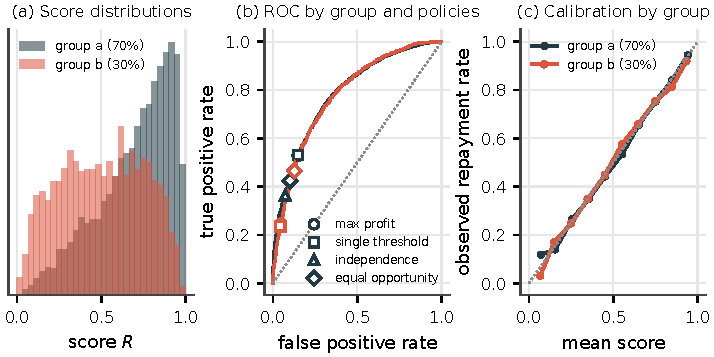
\includegraphics[width=\textwidth]{ch03/fairness_credit}
\caption{The credit-scoring case study, on test data. (a) Distribution of the score in each group.
(b) ROC curve of each group with the operating points of the four policies, whose thresholds were
chosen on validation data. (c) The score is calibrated
in both groups (sufficiency).}
\label{fig:fairnesscredit}
\end{figure}

What is the purpose of a fairness\index{fairness} criterion here? Independence would lend at the same rate in
both groups, regardless of the individuals' ability to repay, and loans that end in default can
harm the people who receive them. Imposing a criterion on a one-shot decision can even make things
worse in the long run for the group it aims to protect \citep{liu2018delayed}; directly optimising
the long-term benefit of the decisions may be a more effective intervention\index{intervention}. An alternative view
is that the criteria have \emph{diagnostic} value: the different true positive rates in our
example show that creditworthy members of group $b$ bear a much higher cost of the classification
(they are refused credit more often), a cost that is not reflected in the profit function that
the bank optimised.

% ---------------------------------------------------------------------
\section{Causality}\label{sec:causality}

Causal reasoning is a conceptual and technical framework for questions about the effect of
hypothetical actions or interventions\index{intervention}: what would happen if we did something, and which action
caused an event? Causal inference\index{causality} gives us a formal language to ask these questions, but it does
not make it easy to choose the right question, nor does it trivialise finding and interpreting the
answer. In the context of fairness\index{fairness}, causality serves three purposes: to understand the limitations
of observational criteria, to design interventions that achieve a desired effect, and to reason
about discrimination, which is itself a causal notion (\emph{because of} their sex, their
ethnicity\dots).

\subsection{The limits of observation}

In 1973 the University of California, Berkeley, admitted 44\% of the 8442 men and 35\% of the
4321 women who applied to its graduate programmes. Was there a gender bias? Admissions were
decided by each department, and \citet{bickel1975sex} looked at the departments separately.
\Cref{lst:berkeley} shows the six largest ones: women were admitted at a similar or higher rate
in four of the six, yet in aggregate the gap persists (44.5\% against 30.4\%). This reversal is an
instance of \emph{Simpson\index{Simpson's paradox|textbf}'s paradox} \citep{simpson1951interpretation}.

\begin{pylisting}[label={lst:berkeley}]{Simpson's paradox in the Berkeley admissions data}
import pandas as pd

# Six largest departments, UC Berkeley 1973 (Bickel et al., 1975)
d = pd.DataFrame({"dept": list("ABCDEF"),
                  "men": [825, 560, 325, 417, 191, 373],
                  "men_adm": [512, 353, 120, 138, 53, 22],
                  "women": [108, 25, 593, 375, 393, 341],
                  "women_adm": [89, 17, 202, 131, 94, 24]})
d["men_rate"], d["women_rate"] = d.men_adm / d.men, d.women_adm / d.women
cols = ["dept", "men", "men_rate", "women", "women_rate"]
print(d[cols].round(2).to_string(index=False))
print(f"aggregate:   men {d.men_adm.sum() / d.men.sum():.3f}   "
      f"women {d.women_adm.sum() / d.women.sum():.3f}")
w = (d.men + d.women) / (d.men + d.women).sum()          # department mix of all applicants
men_adj, women_adj = (w * d.men_rate).sum(), (w * d.women_rate).sum()
print(f"adjusted:    men {men_adj:.3f}   women {women_adj:.3f}")
\end{pylisting}
\begin{pyoutput}
dept  men  men_rate  women  women_rate
   A  825      0.62    108        0.82
   B  560      0.63     25        0.68
   C  325      0.37    593        0.34
   D  417      0.33    375        0.35
   E  191      0.28    393        0.24
   F  373      0.06    341        0.07
aggregate:   men 0.445   women 0.304
adjusted:    men 0.387   women 0.430
\end{pyoutput}

The explanation is that women applied more often to departments with low admission rates (C to
F), while men applied mostly to departments A and B, which admitted most of their applicants.
If we weight the department-specific rates by the overall distribution of applicants across
departments (the last line of the output, explained in \cref{sec:adjustment}), women's admission
rate is 43.0\% and men's 38.7\%. But the data cannot tell us \emph{why} women applied to more
competitive departments: because of their interests, because some departments advertised in ways
that discouraged women, because of a hostile climate, or for other reasons. These scenarios have
different interpretations and consequences, and they cannot be distinguished with the data at
hand. Causal models help to design new studies and to decide which variables to measure and which
to include or exclude in an analysis.

\subsection{Structural causal models}

A \emph{structural causal model\index{structural causal model|textbf}} (SCM) is a program that generates a distribution from independent
noise variables through a sequence of assignments \citep{pearl2009causality,peters2017elements}.

\begin{definition}{Structural causal model}{scm}
A structural causal model $M$ consists of variables $X_1,\dots,X_d$ and assignments
\begin{equation}
  X_i:=f_i(P_i,U_i),\qquad i=1,\dots,d,
\end{equation}
where $P_i\subseteq\{X_1,\dots,X_d\}$ are the \emph{parents} (direct causes) of $X_i$ and the
\emph{noise variables} $U_1,\dots,U_d$ are jointly independent exogenous factors. The \emph{causal
graph\index{causal graph|textbf}} has one node per variable and an edge from each parent to its child; we assume it is
acyclic. Executing the assignments in order generates a joint distribution $P_M$.
\end{definition}

\begin{example}{Exercise, overweight and heart disease}{heart}
An individual exercises regularly with probability 1/2. With probability 1/3 they have a latent
disposition to overweight, which manifests itself only without regular exercise; and without
exercise, heart disease occurs with probability 1/3. With $X$ the indicator of regular exercise,
$W$ of overweight and $H$ of heart disease, and independent noise $U_1\sim B(1/2)$,
$U_2\sim B(1/3)$, $U_3\sim B(1/3)$:
\begin{equation*}
  X:=U_1,\qquad W:=\begin{cases}0 & \text{if } X=1\\ U_2 & \text{otherwise}\end{cases},\qquad
  H:=\begin{cases}0 & \text{if } X=1\\ U_3 & \text{otherwise.}\end{cases}
\end{equation*}
Exercise prevents both overweight and heart disease, and without exercise the two are
independent. The probability of heart disease is $P_M\{H=1\}=1/2\cdot1/3=1/6$. Among overweight
people, who never exercise, it is $P_M\{H=1\mid W=1\}=1/3$. Does overweight cause heart disease in
this model? Replace the assignment of $W$ by $W:=1$, keeping the rest: the probability of heart
disease is still $1/6$, because $H$ does not depend on $W$ (\cref{lst:heart}). Observing that
someone is overweight tells us that their risk is higher, but making them lose weight would not
change it: overweight and heart disease share a common cause.
\end{example}

\begin{pylisting}[label={lst:heart}]{Conditioning versus intervening in the heart disease model}
import numpy as np

rng = np.random.default_rng(0)
n = 1_000_000

def heart_model(do_W=None):
    """Structural causal model: exercise X, overweight W and heart disease H."""
    U1, U2, U3 = rng.random(n) < 1 / 2, rng.random(n) < 1 / 3, rng.random(n) < 1 / 3
    X = U1
    W = np.where(X, False, U2) if do_W is None else np.full(n, do_W)
    H = np.where(X, False, U3)
    return X, W, H

X, W, H = heart_model()
print(f"P(H = 1)              = {H.mean():.3f}   (exact 1/6 = 0.167)")
print(f"P(H = 1 | W = 1)      = {H[W].mean():.3f}   (exact 1/3 = 0.333)")
_, _, H_do = heart_model(do_W=True)
print(f"P(H = 1 | do(W := 1)) = {H_do.mean():.3f}   (W does not cause H)")
\end{pylisting}
\begin{pyoutput}
P(H = 1)              = 0.167   (exact 1/6 = 0.167)
P(H = 1 | W = 1)      = 0.335   (exact 1/3 = 0.333)
P(H = 1 | do(W := 1)) = 0.167   (W does not cause H)
\end{pyoutput}

A causal model is a collection of assumptions about how variables interact. When we talk about
causes and effects \emph{in a model} we do not claim that they hold in the real world; different
models describe different hypothetical scenarios and serve as a basis for discussion.

\subsection{Causal graphs: forks, chains and colliders}

What matters in a causal graph\index{causal graph} are the paths that are present and absent. A node is a \emph{direct
cause} of its children and an \emph{indirect cause} of all its descendants. Three basic structures
(\cref{fig:structures}) determine how information flows and what happens when we condition on
(``control for'') a variable $Z$:
\begin{itemize}
  \item a \emph{fork\index{fork|textbf}} $X\leftarrow Z\rightarrow Y$: $Z$ is a common cause, a \emph{confounder\index{confounder|textbf}},
        that makes $X$ and $Y$ correlated even if neither causes the other (exercise in
        \cref{ex:heart}). Conditioning on $Z$ removes the spurious association;
  \item a \emph{chain} $X\rightarrow Z\rightarrow Y$: $Z$ is a \emph{mediator\index{mediator|textbf}} that transmits part
        of the effect of $X$. Conditioning on $Z$ removes the part of the effect that goes through
        it;
  \item a \emph{collider\index{collider|textbf}} $X\rightarrow Z\leftarrow Y$: $Z$ is a common effect. $X$ and $Y$ are
        independent, but conditioning on $Z$ \emph{creates} an association between them. Two
        unrelated diseases become negatively correlated among hospital patients, because having
        either one is enough to be admitted; and an admission test may seem uninformative when it
        is studied only among admitted students, who were selected partly because of it.
\end{itemize}

\begin{figure}[htbp]
\centering
\begin{tikzpicture}[font=\small\sffamily,
  v/.style={circle,draw=edmnavy,fill=edmnavy!8,minimum size=7mm,inner sep=0pt},
  hl/.style={v,fill=edmbronze!25,draw=edmbronze},
  arr/.style={-{Stealth[length=2mm]},edmnavy,thick}]
  \begin{scope}
    \node[v] (x) at (0,0) {$X$}; \node[v] (y) at (2,0) {$Y$}; \node[hl] (z) at (1,1.2) {$Z$};
    \draw[arr] (z) -- (x); \draw[arr] (z) -- (y); \draw[arr,dashed] (x) -- (y);
    \node at (1,-0.8) {(a) fork: $Z$ confounds};
  \end{scope}
  \begin{scope}[xshift=3.6cm]
    \node[v] (x) at (0,0) {$X$}; \node[hl] (z) at (1,1.2) {$Z$}; \node[v] (y) at (2,0) {$Y$};
    \draw[arr] (x) -- (z); \draw[arr] (z) -- (y); \draw[arr,dashed] (x) -- (y);
    \node at (1,-0.8) {(b) chain: $Z$ mediates};
  \end{scope}
  \begin{scope}[xshift=7.2cm]
    \node[v] (x) at (0,0) {$X$}; \node[v] (y) at (2,0) {$Y$}; \node[hl] (z) at (1,1.2) {$Z$};
    \draw[arr] (x) -- (z); \draw[arr] (y) -- (z);
    \node at (1,-0.8) {(c) collider};
  \end{scope}
  \begin{scope}[xshift=10.8cm]
    \node[v] (x) at (1,1.2) {$X$}; \node[v] (w) at (0,0) {$W$}; \node[v] (h) at (2,0) {$H$};
    \draw[arr] (x) -- (w); \draw[arr] (x) -- (h);
    \node at (1,-0.8) {(d) heart model};
  \end{scope}
\end{tikzpicture}
\caption{Basic causal structures. Dashed edges are possible direct effects. (d) The causal graph
of \cref{ex:heart}: exercise $X$ is a common cause of overweight $W$ and heart disease $H$.}
\label{fig:structures}
\end{figure}

\Cref{lst:adjustment} simulates the three structures with linear models in which the true effect
of $X$ on $Y$ is known. In the fork, the naive regression of $Y$ on $X$ doubles the effect (2.00
instead of 1) and adjusting for $Z$ recovers it. In the chain, the naive regression gives the
total effect (4) and adjusting for the mediator leaves only the direct effect (1). In the collider,
$X$ has no effect on $Y$ and the naive regression says so, but adjusting for $C$ creates a
spurious effect of $-0.5$.

\begin{pylisting}[label={lst:adjustment}]{Adjusting for a confounder, a mediator and a collider}
import numpy as np
from sklearn.linear_model import LinearRegression

rng = np.random.default_rng(1)
n = 100_000
coef = lambda cols, y: LinearRegression().fit(np.column_stack(cols), y).coef_[0]
noise = lambda: rng.normal(size=n)

# (a) fork: Z is a common cause of X and Y; the effect of X on Y is 1
Z = noise()
X = Z + noise()
Y = X + 2 * Z + noise()
print(f"fork:     naive {coef([X], Y):.2f}   adjusting for Z {coef([X, Z], Y):.2f}")
# (b) chain: X -> M -> Y plus a direct effect; total 1 + 2 * 1.5 = 4, direct 1
X = noise()
M = 2 * X + noise()
Y = X + 1.5 * M + noise()
print(f"mediator: naive {coef([X], Y):.2f}   adjusting for M {coef([X, M], Y):.2f}")
# (c) collider: X -> C <- Y; X has no effect on Y
X = noise()
Y = noise()
C = X + Y + noise()
print(f"collider: naive {coef([X], Y):.2f}   adjusting for C {coef([X, C], Y):.2f}")
\end{pylisting}
\begin{pyoutput}
fork:     naive 2.00   adjusting for Z 1.00
mediator: naive 4.00   adjusting for M 1.01
collider: naive 0.00   adjusting for C -0.50
\end{pyoutput}

\subsection{Interventions and the do-operator}

Structural causal models\index{structural causal model} formalise the effect of hypothetical actions. Given a model $M$, we can
replace an assignment $X:=f(P,U)$ by another one, most often a constant, $X:=x$. The resulting
model $M[X:=x]$ removes the influence of the parents of $X$, and the probability of an event $E$
after the intervention\index{intervention} is written
\begin{equation}
  P\{E\mid\mathrm{do}(X:=x)\}=P_{M[X:=x]}(E).
\end{equation}
This notation, the \emph{do-operator}, resembles a conditional probability, but an action is
fundamentally different from an observation. The \emph{causal effect} of the action $X:=x$ on $Y$
is the distribution of $Y$ in $M[X:=x]$; for a binary $X$ we usually summarise it by the
\emph{average treatment effect}
\begin{equation}
  \mathrm{ATE}=\E_{M[X:=1]}[Y]-\E_{M[X:=0]}[Y].
\end{equation}
In general $P\{Y=y\mid\mathrm{do}(X:=x)\}\neq P\{Y=y\mid X=x\}$, and we say that $X$ and $Y$ are
\emph{confounded} when the causal effect differs from the corresponding conditional probability.

\subsection{Adjustment and the backdoor criterion}\label{sec:adjustment}

When $X$ and $Y$ are confounded, the effect of an intervention\index{intervention} can sometimes be computed from
observational data. If $Z$ is the set of parents of $X$ (or, more generally, any set of variables
that satisfies the backdoor\index{backdoor criterion} criterion below), the \emph{adjustment formula} gives
\begin{equation}\label{eq:adjustment}
  P\{Y=y\mid\mathrm{do}(X:=x)\}=\sum_{z}P\{Y=y\mid X=x,Z=z\}\,P\{Z=z\}.
\end{equation}
In words, we estimate the effect separately in each stratum of $Z$ and average the results,
weighting each stratum by its share of the \emph{whole} population (not of the treated). The
``adjusted'' line of \cref{lst:berkeley} performs the same computation with $Z$ the department, but there
it is a \emph{descriptive} standardisation to a common distribution of departments: in the causal graph\index{causal graph}
of Berkeley discussed below, the department is a mediator\index{mediator} of sex, not a confounder\index{confounder}, so it is not a valid
adjustment set for the total effect.

A \emph{backdoor path} from $X$ to $Y$ is a path that starts with an edge pointing into $X$. When it is
\emph{open}, it lets information flow from $X$ to $Y$ in a non-causal way and the effect is confounded.
Conditioning on a non-collider\index{collider} on the path blocks it; a collider blocks it unless the collider or one
of its descendants is conditioned on. A set $Z$ satisfies the \emph{backdoor criterion} if it blocks every backdoor
path and contains no descendant of $X$; conditioning on it deconfounds the effect.

Two warnings apply. First, the adjustment formula is only valid in the absence of
\emph{unobserved confounding}, variables that are hard to measure or were never recorded, which
remains a major obstacle in practice. Second, it is tempting to control for as many variables as
possible in the hope of removing confounding, but controlling for mediators or colliders is
harmful (\cref{lst:adjustment}). The experimental alternative is the \emph{randomised controlled
trial}: subjects are randomly assigned to a treatment or a control group (ideally without knowing
which, both they and the staff), which removes every incoming edge into the treatment variable, so
that any difference in the outcome can be attributed to the treatment.

\subsection{Graphical discrimination analysis}

Let us return to Berkeley with a causal model with three variables: sex $A$, department choice
$Z$ and admission $Y$ (\cref{fig:berkeley}). Admission depends on the department and possibly on
sex ($Z\rightarrow Y$, $A\rightarrow Y$), and the data show that department choice depends on sex
($A\rightarrow Z$). The argument of \citet{bickel1975sex} had two parts: there is no evidence of a
\emph{direct} effect of sex on admission favouring men, and the \emph{indirect} effect through
department choice should not count as discrimination.

\begin{figure}[htbp]
\centering
\begin{tikzpicture}[font=\small\sffamily,
  v/.style={circle,draw=edmnavy,fill=edmnavy!8,minimum size=8mm,inner sep=0pt},
  arr/.style={-{Stealth[length=2mm]},edmnavy,thick}]
  \node[v] (a) at (0,0) {$A$};
  \node[v] (z) at (2.4,1.3) {$Z$};
  \node[v] (y) at (4.8,0) {$Y$};
  \node[v,dashed,draw=edmcoral,fill=edmcoral!10] (r) at (4.8,2.6) {$R$};
  \draw[arr] (a) -- node[above left,font=\scriptsize] {choice} (z);
  \draw[arr] (z) -- (y);
  \draw[arr] (a) -- node[below,font=\scriptsize] {direct effect} (y);
  \draw[arr,dashed,edmcoral] (r) -- (z);
  \draw[arr,dashed,edmcoral] (r) -- (y);
  \node[align=left,anchor=west,font=\scriptsize] at (5.5,1.2)
    {$A$: sex\\$Z$: department chosen\\$Y$: admission\\$R$: e.g.\ state of residence\\(hypothetical confounder)};
\end{tikzpicture}
\caption{A causal graph for the Berkeley admissions. If an unobserved variable $R$ influences both
department choice and admission, conditioning on $Z$ opens the path $A\rightarrow Z\leftarrow
R\rightarrow Y$ and the direct effect of $A$ can no longer be estimated by comparing admission
rates within departments.}
\label{fig:berkeley}
\end{figure}

\paragraph{Direct effect} To isolate the direct effect we must disable every path between $A$ and
$Y$ except the direct edge, which suggests holding the department fixed and comparing admission
rates within departments, as Bickel did. This is valid only if department choice and admission are
not confounded. If some other variable, say the state of residence $R$, influenced both, then $Z$
would be a collider\index{collider} on the path $A\rightarrow Z\leftarrow R\rightarrow Y$, and conditioning on it
would open a non-causal path. Assuming no such confounding\index{confounder}, the data show no direct effect of sex
against women. But the direct effect is a poor measure of discrimination on its own, since it
cannot detect discrimination that operates through other variables.

\paragraph{Indirect paths} Department choice may itself be shaped by discrimination: departments
may advertise their programmes in ways that discourage women, have a history of hostile behaviour,
or be feared to discriminate. Accepting the indirect path as non-discriminatory amounts to
asserting that all these scenarios are implausible. Seemingly innocuous mediating paths can hide
discriminatory practices: in \emph{Griggs v.\ Duke Power Co.} (1971), the US Supreme Court struck
down a requirement of a high-school diploma for jobs where it was not related to performance,
because it excluded disproportionately many Black applicants. We have to discuss carefully which
pathways count as evidence for or against discrimination. Discrimination can also be
\emph{structural}, embedded in the way society is organised, which models that describe how a
decision maker responds to information about individuals can hardly capture.

\subsection{Counterfactuals}

A fully specified structural causal model\index{structural causal model} can answer questions more delicate than the effect of
an action. ``Would I have avoided the traffic jam had I taken the other route this morning?'' is a
\emph{counterfactual\index{counterfactual|textbf}} question: it asks about an alternative to what actually happened, taking into
account what we observed.

\begin{example}{Which route?}{traffic}
Every morning we choose route 0 or 1 at random, $X:=U_X\sim B(1/2)$. A morning is slow ($Y=1$) if
it is a bad day ($U=1$, both routes are slow) or if there is an accident on the chosen route
($U_0=1$ or $U_1=1$), with $U,U_0,U_1\sim B(1/2)$ independent: $Y:=\max(U,U_0)$ if $X=0$ and
$Y:=\max(U,U_1)$ if $X=1$. This morning we took route 1 and it was slow
($X=1$, $Y=1$). Would route 0 have been better?

The naive answer uses the intervention\index{intervention}: $P\{Y=0\mid\mathrm{do}(X:=0)\}=P\{U=0,U_0=0\}=1/4$. But
this ignores what we observed. The evidence $\{X=1,Y=1\}$ leaves three equally likely settings of
$(U,U_1)$: $(1,0)$, $(1,1)$ and $(0,1)$, so it was a bad day with probability $2/3$. Route 0 would
have been fast only if it was a good day ($1/3$) and there was no accident on route 0 ($1/2$):
the counterfactual probability is $1/6$. The observation biases the distribution of the noise
variables (\cref{lst:traffic}).
\end{example}

\begin{pylisting}[label={lst:traffic}]{Intervention versus counterfactual in the traffic example}
import numpy as np

rng = np.random.default_rng(2)
n = 2_000_000
# bad day, accident on route 0 / 1, route choice
U, U0, U1, UX = rng.random((4, n)) < 0.5

def morning(X, U, U0, U1):
    """Y = 1 means a slow morning: a bad day or an accident on the chosen route."""
    return np.where(X == 0, U | U0, U | U1)

X = UX.astype(int)
Y = morning(X, U, U0, U1)
p_do = np.mean(morning(0, U, U0, U1) == 0)
print(f"P(Y=0 | do(X:=0))          = {p_do:.3f}  (exact 1/4)")
E = (X == 1) & (Y == 1)                                  # evidence: route 1, slow morning
print(f"P(U=1 | X=1, Y=1)          = {U[E].mean():.3f}  (exact 2/3)")
cf = morning(0, U[E], U0[E], U1[E])                      # abduction, action, prediction
print(f"P(Y_(X:=0) = 0 | X=1, Y=1) = {np.mean(cf == 0):.3f}  (exact 1/6)")
\end{pylisting}
\begin{pyoutput}
P(Y=0 | do(X:=0))          = 0.250  (exact 1/4)
P(U=1 | X=1, Y=1)          = 0.666  (exact 2/3)
P(Y_(X:=0) = 0 | X=1, Y=1) = 0.167  (exact 1/6)
\end{pyoutput}

In general, given a model $M$, an observed event $E$, an action $X:=x$ and a target variable $Y$,
the counterfactual $Y_{X:=x}(E)$ is computed in three steps \citep{pearl2009causality}:
\begin{enumerate}
  \item \emph{abduction\index{abduction|textbf}}: condition the distribution of the noise variables $U=(U_1,\dots,U_d)$ on
        the event $E$, obtaining a biased distribution $U'$;
  \item \emph{action}: perform the intervention, obtaining $M'=M[X:=x]$;
  \item \emph{prediction}: compute $Y$ in $M'$ using $U'$ as the random seed.
\end{enumerate}
The result is the value $Y$ would have taken had $X$ been set to $x$, in the circumstances
described by $E$.

\subsection{Potential outcomes}

A second framework for causal inference\index{causality}, popular in statistics, economics and medicine, is that of
\emph{potential outcomes} \citep{rubin1974estimating,imbens2015causal}. It assumes that every unit
$u$ (a person, a school, a day) has a potential outcome $Y_x(u)$ for every possible value $x$ of the
treatment; for a binary treatment, $Y_0(u)$ and $Y_1(u)$. Only one of them is observed:
\begin{equation}
  Y(u)=Y_0(u)\,\bigl(1-T(u)\bigr)+Y_1(u)\,T(u).
\end{equation}
Causal inference then becomes a missing-data problem: a typical query is the average effect
$\E[Y_1-Y_0]$, and estimating it means filling in the missing potential outcomes. This becomes
possible under well-established conditions:
\begin{itemize}
  \item \emph{SUTVA} (stable unit treatment value assumption): the treatment of one unit does not
        change the outcome of other units;
  \item \emph{consistency}: the observed outcome equals the potential outcome of the treatment
        actually received;
  \item \emph{ignorability}: the potential outcomes are independent of the treatment given some
        set of deconfounding variables $Z$, $T\perp(Y_0,Y_1)\mid Z$.
  \item \emph{positivity} (overlap): every value of the treatment occurs with positive probability
        at the covariate values of the target population, $0<P(T=1\mid Z=z)<1$; SUTVA also requires
        well-defined treatments, without hidden versions that matter.
\end{itemize}
The potential outcomes framework is generally easier to apply than full structural models, but
its ease can also lead to abuse: applying effect estimators when these assumptions do not hold
produces false results, and possibly ineffective or harmful interventions\index{intervention} \citep{hernan2020causal}.

\subsection{Mediation and path-specific effects}

\emph{Mediation analysis\index{mediation analysis|textbf}} decomposes a total causal effect into the contributions of different
paths \citep{pearl2001direct}. Consider a treatment $X$, a mediator\index{mediator} $Z$ and an outcome $Y$, with
edges $X\rightarrow Z\rightarrow Y$ and $X\rightarrow Y$. The \emph{total effect}
$\E[Y\mid\mathrm{do}(X:=1)]-\E[Y\mid\mathrm{do}(X:=0)]$ includes both pathways. The \emph{controlled
direct effect\index{controlled direct effect|textbf}} holds the mediator at a fixed level $z$,
\begin{equation}
  \mathrm{CDE}(z)=\E[Y\mid\mathrm{do}(X:=1,Z:=z)]-\E[Y\mid\mathrm{do}(X:=0,Z:=z)],
\end{equation}
and does not need counterfactuals. Sometimes it is more meaningful to let the mediator take the
value it would have had \emph{without} treatment; this needs counterfactuals and gives the
\emph{natural direct effect\index{natural direct effect|textbf}} and the \emph{natural indirect effect\index{natural indirect effect|textbf}},
\begin{equation}
  \mathrm{NDE}=\E\bigl[Y_{X:=1,\,Z:=Z_{X:=0}}\bigr]-\E[Y_{X:=0}],\qquad
  \mathrm{NIE}=\E\bigl[Y_{X:=0,\,Z:=Z_{X:=1}}\bigr]-\E[Y_{X:=0}].
\end{equation}
The \emph{pure} natural direct effect (PNDE) holds the mediator at its untreated value and changes
the treatment from zero to one, $\E[Y_{1,Z_0}]-\E[Y_{0,Z_0}]$; the \emph{pure} natural indirect effect (PNIE)
holds the treatment at zero and changes the mediator from its untreated to its treated value,
$\E[Y_{0,Z_1}]-\E[Y_{0,Z_0}]$. They add up to the total effect in the linear,
additive example of this section, but not in general: with $Z:=X$ and $Y:=XZ$ the total effect is 1 and
both pure effects are 0, because the effect is an interaction. A general additive decomposition pairs
the pure natural direct effect with the \emph{total} natural indirect effect,
$\E[Y_{1,Z_1}]-\E[Y_{1,Z_0}]$. Identifying natural effects from observational data requires stronger
assumptions than the total effect, including the absence of confounding\index{confounder} between mediator and outcome
\citep{pearl2001direct}.
In a linear model $Z:=0.8X+U_Z$, $Y:=0.5X+Z+U_Y$, the total effect is $0.5+0.8\cdot1=1.3$, the
natural direct effect 0.5 and the natural indirect effect 0.8. In the absence of confounding,
natural effects can be estimated from observational data, and counterfactuals allow us to compute
other path-specific\index{path-specific effect} effects and to design decision rules\index{decision rules} that eliminate the effects we deem
undesirable.

\subsection{Counterfactual fairness}

Counterfactuals also suggest a fairness\index{fairness} criterion. With features $X$, sensitive attribute\index{protected attribute} $A$ and
predictor $\hat Y$, a predictor is \emph{counterfactually fair} \citep{kusner2017counterfactual}
if, for every individual described by an event $E=\{X=x,A=a\}$ and every alternative value $a'$,
the counterfactual predictions $\hat Y_{A:=a'}(E)$ and $\hat Y_{A:=a}(E)$ have the same
distribution: the prediction would have been the same had the person belonged to another group,
with everything that this change would have implied. The easiest way of satisfying it is to use
only features that are not descendants of $A$ in the causal graph\index{causal graph}.

A common shortcut is \emph{attribute flipping\index{attribute flipping|textbf}}: change the sensitive attribute of a record, leave
everything else unchanged, and compare the predictions. In the lawsuit over admissions at Harvard
College, an expert report estimated the effect of race by changing it in a statistical model of
admissions while keeping the other characteristics of the applicants fixed. Flipping the sensitive
attribute while holding the other model inputs fixed generally fails to represent its total counterfactual effect
when those inputs are affected descendants of the attribute, which is plausible for race or gender, since they
influence many other features. It can be valid under additional structural assumptions: the absence of affected
descendants among the inputs of the model is a sufficient condition. Otherwise, the intervention\index{intervention} being estimated
must be stated explicitly. We cannot meaningfully
talk about counterfactuals without being clear about how the variables interact.

\subsection{The validity of causal models}

A valid causal model is one that represents scientific knowledge \citep{pearl2018book}. Causal
statements without grounding in established knowledge are better thought of as convenient
mathematical fictions, and the line between the two is often blurry. Mistaking a mediator\index{mediator} for a
confounder\index{confounder}, for instance, leads to adjusting for a variable that should be left alone, one of the
most serious errors in causal inference\index{causality}. Additional difficulties arise when the variables are
human categories: socially constructed categories such as race or gender are hard to delimit and
to ``intervene'' on, the variables of social systems are rarely modular (changing one changes the
mechanisms of others), and the concepts we reason about may not be stable enough for the claims we
make.

% =====================================================================
\section{Interpretable machine learning}\label{sec:interpretability}

Machines already exceed people in many prediction tasks, in speed, reproducibility and scale. The
price is that the knowledge they use is hidden in increasingly complex models: deep neural
networks, random forests\index{random forest}, ensembles\index{ensemble}. \emph{Interpretability\index{interpretability|textbf}} is the degree to which a human can
understand the cause of a decision \citep{miller2019explanation}; a model is more interpretable
than another if its decisions are easier to comprehend. Interpretable machine learning can imply,
but does not necessarily require, giving a human-style explanation of each prediction.

\subsection{Why interpretability matters}

A single metric, such as accuracy, is an incomplete description of most real-world tasks. Often
we want to know \emph{why} a prediction was made, and we may be willing to pay for that knowledge
with some accuracy, because the answer helps us to understand the problem, the data and how the
model might fail. The need for explanations comes from an \emph{incompleteness} of the problem
formalisation \citep{doshivelez2017towards}: the objective that the model optimises is never
exactly what we care about. Interpretability helps to:
\begin{itemize}
  \item \emph{learn} from the model, which matters for science;
  \item ensure \emph{safety}: a model that predicted the risk of death of pneumonia patients learned
        that asthma \emph{lowered} the risk, because asthmatic patients were treated more
        aggressively in the training data; deployed without understanding, it would have
        denied them care \citep{caruana2015intelligible};
  \item detect \emph{bias} (does the loan model discriminate against a minority?) and check other
        properties: fairness\index{fairness}, privacy, robustness, causality\index{causality};
  \item gain \emph{trust} and social acceptance, and manage the social interaction between the
        system and its users;
  \item \emph{debug} and audit models.
\end{itemize}
Explanations are not always needed: not when the consequences of errors are mild (a movie
recommender\index{recommender system}), not for problems that have been studied for a long time (optical character
recognition), and not when explaining would let people game the system. But the more a decision
affects a person's life, the more important it is that the machine can explain it.

\subsection{A taxonomy of interpretability methods}

Interpretability methods can be classified along several dimensions:
\begin{itemize}
  \item \emph{intrinsic} or \emph{post hoc}: intrinsically interpretable models (short trees,
        sparse linear models) are understood by inspecting them; post-hoc methods analyse a model
        after training, and can also be applied to interpretable models;
  \item \emph{model-specific} or \emph{model-agnostic}: the first are limited to one class of
        models (the weights of a linear model); the second work with any model, only through its
        inputs and outputs;
  \item \emph{local} or \emph{global}: explaining one prediction or the whole model;
  \item the \emph{outcome} of the method: a feature summary statistic (an importance), a feature
        summary visualisation (a partial dependence\index{partial dependence plot} plot), model internals (learned weights), data
        points (a counterfactual, a prototype\index{prototypes and criticisms}), or an intrinsically interpretable model that
        approximates the black box.
\end{itemize}
The \emph{scope} of the interpretation ranges from algorithm transparency (how the algorithm learns
a model, without reference to a particular model), through global holistic interpretability (how
the trained model makes its decisions as a whole, very hard beyond a few dimensions) and global
interpretability on a modular level (how parts of the model, such as a weight or a branch,
influence predictions), to local interpretability for a single prediction or for a group of
predictions.

\subsection{Evaluating interpretability}

There is no consensus on how to measure interpretability. \citet{doshivelez2017towards} distinguish
three levels of evaluation: \emph{application-grounded} (put the explanation into the product and
let the end users test it on the real task), \emph{human-grounded} (simpler experiments with lay
people, for instance choosing the better of two explanations) and \emph{functionally grounded}
(proxies that need no humans, such as the depth of a tree or the number of rules). Other proxies
are sparsity, monotonicity, the length of the explanation, and the cognitive processing time.

\subsection{Human-friendly explanations}

An explanation is the answer to a why-question. Research in the social sciences shows what people
expect from one \citep{miller2019explanation}:
\begin{itemize}
  \item explanations are \emph{contrastive}: people ask why this prediction was made \emph{instead
        of another}, and think in counterfactual terms. A good explanation compares with a
        reference, which depends on the application;
  \item explanations are \emph{selective}: people prefer one or two causes rather than a complete
        list;
  \item explanations are \emph{social}: they depend on the explainer, the receiver and the context;
  \item explanations focus on the \emph{abnormal}: rare causes that changed the outcome a lot are
        preferred, and must be included;
  \item explanations should be \emph{truthful} (faithful\index{faithfulness} to the model), \emph{coherent with the
        prior beliefs} of the receiver, a psychological expectation (people tend to ignore information
        that contradicts them) that must never override fidelity\index{fidelity} to the model and to the evidence,
        and \emph{general and probable} (a cause that explains many events is a good explanation,
        which contradicts the preference for abnormal causes).
\end{itemize}
If we need all the factors that contributed to a prediction (for legal reasons, or to debug a
model) we do not want a human-style explanation but a complete attribution.

% ---------------------------------------------------------------------
\section{Interpretable models}\label{sec:intmodels}

The most straightforward way of obtaining interpretable models is to use algorithms that produce
them. \Cref{tab:intmodels} summarises their properties: a model is \emph{linear} if the
association between features and target is linear, and \emph{monotone} if increasing a feature
always moves the prediction in the same direction.

\begin{table}[htbp]
\centering\small
\caption{Properties of common interpretable models. Linearity and additivity depend on the output scale
(prediction, logit, probability) and on the representation of the features.}\label{tab:intmodels}
\begin{tabularx}{\textwidth}{@{}l>{\raggedright\arraybackslash}X>{\raggedright\arraybackslash}p{2.7cm}>{\raggedright\arraybackslash}p{3.6cm}@{}}
\toprule
Model & Scale or representation & Monotone & Interactions\\
\midrule
Linear regression & prediction linear in the inputs & yes, per input & only if terms are added\\
Logistic regression & logit linear in the inputs; the probability is not additive & yes, per input & only if terms are added to the logit\\
Decision tree & partitions of the input space & not in general & yes\\
Decision rules & conditions on the inputs & not in general & yes\\
RuleFit & linear in the inputs and in the expanded rule features & not in general & yes, through the rules\\
Naive Bayes & log-odds add the log-likelihood ratios of the features & not in general & none in the log-odds, under its assumption\\
$k$-nearest neighbours & neighbourhoods of the input space & not in general & yes\\
\bottomrule
\end{tabularx}
\end{table}

\subsection{Linear regression}

A linear model predicts the target as a weighted sum of the features,
$\hat y=\beta_0+\beta_1x_1+\dots+\beta_px_p$. Its understandability is why linear models are so
widespread in medicine, sociology, psychology and many other quantitative fields. Their usual
interpretation relies on assumptions that are often not satisfied: \emph{linearity} (non-linear
effects and interactions must be added by hand), \emph{homoscedasticity} (constant error variance),
\emph{independence} of the examples, \emph{fixed} features measured without error, and no perfect
\emph{collinearity}. Exact classical confidence intervals\index{confidence interval} also require Gaussian errors; asymptotic, robust or
bootstrap\index{bootstrap} inference may be appropriate in other settings. Perfect collinearity prevents a unique identification
of the coefficients, while strongly correlated features make the individual weights very uncertain.

The weights are interpreted with simple templates:
\begin{itemize}
  \item numerical feature: an increase of $x_k$ by one unit increases the expected outcome by
        $\beta_k$ units, \emph{given that all the other features stay the same};
  \item binary or categorical feature (one-hot encoded): a change from the reference level to
        another level changes the expected outcome by the weight of that level;
  \item intercept $\beta_0$: the expected outcome when all numerical features are zero and the
        categorical ones are at their reference level; usually meaningless unless the features are
        centred.
\end{itemize}
The coefficient of determination\index{coefficient of determination@coefficient of determination ($R^2$)} $R^2=1-\mathrm{SSE}/\mathrm{SST}$ (\cref{sec:regression}) tells how
much of the variance of the target the model explains; since it increases with the number of
features even if they are useless, the \emph{adjusted} version is preferred,
\begin{equation}
  \bar R^2=1-(1-R^2)\,\frac{n-1}{n-p-1},
\end{equation}
with $n$ examples and $p$ features. Training $R^2$ cannot decrease when nested
least-squares models add features on the same data, which guarantees nothing on test data. A low $R^2$ limits the
predictive explanatory power of a model, but does not by itself invalidate the interpretation of its coefficients:
with $y=0.1x$ plus noise of unit variance, $R^2$ is about 0.01, yet the slope can be estimated precisely with
enough data.

The weights are best displayed in a \emph{weight plot}, with their confidence intervals, after
standardising the features so that the weights are comparable. An \emph{effect plot} shows, for
each feature, the distribution over the data of the effects $\beta_jx_{ij}$, the contributions of
the feature to the predictions, and allows a single prediction to be explained by placing its
effects against those distributions. \Cref{fig:linear} and \cref{lst:diabetes} use the diabetes
data of \cref{sec:regression}. The model explains half of the variance ($\bar R^2=0.507$). Body mass
index (bmi), blood pressure (bp) and the serum measurement s5 have clearly positive effects. The
weights of s1 and s2 are large and of opposite sign, but their intervals are very wide and include
zero: the two features are correlated ($r=0.90$), and the model can trade one against the other,
so their individual weights cannot be interpreted. This is multicollinearity in action.

\begin{pylisting}[label={lst:diabetes}]{Weights, confidence intervals and adjusted R2 of a linear model}
import numpy as np
from sklearn.datasets import load_diabetes

data = load_diabetes(as_frame=True)
X, y = data.data, data.target
Xs = (X - X.mean()) / X.std()                            # standardised features
D = np.c_[np.ones(len(Xs)), Xs.values]                   # design matrix with intercept
beta = np.linalg.lstsq(D, y.values, rcond=None)[0]
res = y.values - D @ beta
n, p = D.shape
se = np.sqrt(np.diag(res @ res / (n - p) * np.linalg.inv(D.T @ D)))   # standard errors
r2 = 1 - res @ res / np.sum((y - y.mean()) ** 2)
print(f"R2 = {r2:.3f}   adjusted R2 = {1 - (1 - r2) * (n - 1) / (n - p):.3f}")
for name, b, s in sorted(zip(X.columns, beta[1:], se[1:]), key=lambda t: -abs(t[1]))[:5]:
    print(f"{name:4s} weight={b:7.2f}   95% CI=[{b - 1.96 * s:7.2f}, {b + 1.96 * s:7.2f}]")
print(f"correlation between s1 and s2: {X.s1.corr(X.s2):.2f}")
\end{pylisting}
\begin{pyoutput}
R2 = 0.518   adjusted R2 = 0.507
s1   weight= -37.72   95% CI=[ -76.61,    1.17]
s5   weight=  35.77   95% CI=[  19.73,   51.82]
bmi  weight=  24.75   95% CI=[  18.54,   30.96]
s2   weight=  22.70   95% CI=[  -8.94,   54.34]
bp   weight=  15.45   95% CI=[   9.34,   21.55]
correlation between s1 and s2: 0.90
\end{pyoutput}

\begin{figure}[htbp]
\centering
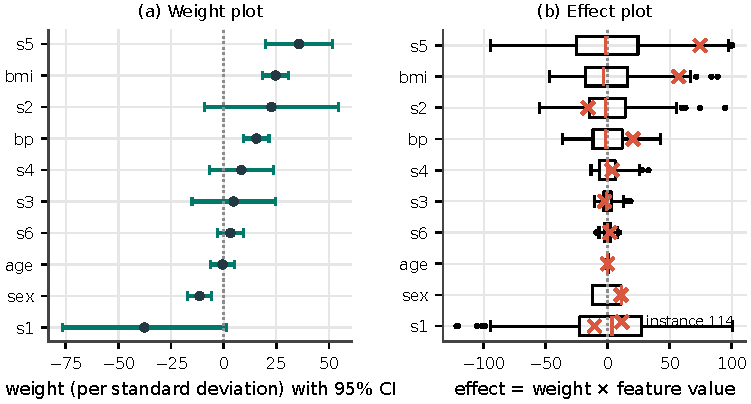
\includegraphics[width=\textwidth]{ch03/linear_weights}
\caption{A linear model of diabetes progression with standardised features. (a) Weights with
95\% confidence intervals. (b) Distribution of the effects of each feature; the crosses are the
effects for the instance with the highest prediction.}
\label{fig:linear}
\end{figure}

Do linear models produce good explanations? They are contrastive, but the reference is an instance
with all features at zero, which is meaningless unless the features are centred; they are
selective only if they are sparse (for instance, fitted with a Lasso penalty); and they are exactly faithful\index{faithfulness} to
the linear model, while the scientific or causal validity of their interpretation depends on whether the
relationship really is linear. Their great advantages are simplicity and
generality. Their disadvantages: every non-linearity or interaction must be hand-crafted, their
predictive performance is often not the best, and the interpretation of a weight depends on all
the other features in the model, which can make it counter-intuitive.

\subsection{Logistic regression}

A linear model is not appropriate for classification: it does not output probabilities, it
extrapolates below zero and above one, and it does not extend to more than two classes.
\emph{Logistic regression\index{logistic regression|textbf}} models the probability of the positive class as
\begin{equation}
  P(y=1\mid x)=\frac{1}{1+e^{-(\beta_0+\beta_1x_1+\dots+\beta_px_p)}},
\end{equation}
so the weights no longer act linearly on the probability. Rearranging, we find a linear model for
the \emph{log odds},
\begin{equation}
  \ln\frac{P(y=1\mid x)}{1-P(y=1\mid x)}=\beta_0+\beta_1x_1+\dots+\beta_px_p,
\end{equation}
and increasing $x_j$ by one unit multiplies the \emph{odds} by $e^{\beta_j}$, the \emph{odds
ratio\index{odds ratio|textbf}}. The templates become: for a numerical feature, an increase of one unit changes the odds by
a factor $e^{\beta_j}$, all the other features staying the same; for a binary feature, changing from
the reference level multiplies the odds by $e^{\beta_j}$; the intercept gives the odds $e^{\beta_0}$
of a reference instance.

\begin{pylisting}[label={lst:loans}]{Synthetic loan applications used in several examples}
"""Synthetic loan applications used in the interpretability examples (Unit 3)."""
import numpy as np

FEATURES = ["income", "debt_ratio", "years_job", "prev_default"]

def loan_data(n=5000, seed=3):
    rng = np.random.default_rng(seed)
    income = rng.normal(30, 8, n)                       # thousand EUR per year
    debt = rng.uniform(0, 0.8, n)                       # debt-to-income ratio
    years = rng.integers(0, 30, n).astype(float)        # years in the current job
    prev = (rng.random(n) < 0.15).astype(float)         # previous default (0/1)
    logit = -2 + 0.08 * income - 3 * debt + 0.03 * years - 1.2 * prev
    y = (rng.random(n) < 1 / (1 + np.exp(-logit))).astype(int)     # 1 = repays
    return np.c_[income, debt, years, prev], y
\end{pylisting}

\Cref{lst:odds} fits a logistic regression to the synthetic loan data of \cref{lst:loans}. Each
additional thousand euros of income multiplies the odds of repaying by 1.081 (an 8\% increase);
an increase of the debt ratio by 0.1 multiplies them by $e^{-0.2976}=0.74$; a previous default
divides them by almost three (0.369). For an applicant with a probability of repaying of 0.30,
10,000 more euros of income would raise it to 0.48. As always, these are statements about the
model, and correlation does not imply causation.

\begin{pylisting}[label={lst:odds}]{Odds ratios of a logistic regression}
import numpy as np
from sklearn.linear_model import LogisticRegression
from loans import FEATURES, loan_data

X, y = loan_data()
m = LogisticRegression(C=1e6, max_iter=5000).fit(X, y)      # practically unregularised
for name, b in zip(FEATURES, m.coef_[0]):
    print(f"{name:13s} beta={b:7.3f}   odds ratio exp(beta)={np.exp(b):6.3f}")
odds = 0.3 / 0.7 * np.exp(10 * m.coef_[0][0])               # P(repay)=0.3, +10k EUR income
p_new = odds / (1 + odds)
print(f"an applicant with P(repay)=0.30 earning 10k EUR more: P(repay)={p_new:.2f}")
\end{pylisting}
\begin{pyoutput}
income        beta=  0.078   odds ratio exp(beta)= 1.081
debt_ratio    beta= -2.976   odds ratio exp(beta)= 0.051
years_job     beta=  0.031   odds ratio exp(beta)= 1.032
prev_default  beta= -0.998   odds ratio exp(beta)= 0.369
an applicant with P(repay)=0.30 earning 10k EUR more: P(repay)=0.48
\end{pyoutput}

\subsection{Decision trees}

Linear and logistic models fail when the relationship between features and target is non-linear or
when features interact. Decision trees\index{decision tree}, such as CART \citep{breiman1984classification}, split the data
recursively, choosing at each node the feature and cut-off that best separate the target (minimum
impurity), until a stopping criterion is reached. The interpretation is simple: starting from the
root, each edge selects a subset of the data, and the leaf gives the prediction; all the conditions
on the path are connected by ``and'':
\begin{center}
\textsc{if} feature $x$ is smaller (or bigger) than threshold $c$ \textsc{and} \dots\ \textsc{then}
the predicted outcome is $\hat y_{\text{leaf}}$.
\end{center}
Trees capture interactions naturally, have a natural visualisation, and produce good explanations:
contrastive (``if the feature had been above the threshold, the prediction would have been\dots''),
selective if the tree is short, and simple. Their drawbacks are that linear relationships are
approximated by steps (lack of smoothness), and that trees are \emph{unstable}: small changes in the
training data can produce a completely different tree (\cref{sec:ensembles}), which does not inspire
confidence in their interpretation.

\subsection{Decision rules}

A \emph{decision rule\index{decision rules|textbf}} is an \textsc{if-then} statement with a condition (antecedent) and a
prediction. Decision rules are probably the most interpretable prediction models, provided the
conditions use intelligible features, are short, and there are not too many rules. The usefulness of
a rule is summarised by its \emph{support} or \emph{coverage\index{coverage|textbf}}, the fraction of instances to which its
condition applies, and its \emph{accuracy\index{accuracy|textbf}} or \emph{confidence}, the fraction of those it predicts
correctly (\cref{sec:unsupervised}). Rules can be combined in a \emph{decision list}, which orders
them (the first rule that applies decides), or in a \emph{decision set}, a democracy of rules in
which some may have more voting\index{voting} power; interpretability suffers when several rules of a set apply.

Some algorithms that learn rules are:
\begin{itemize}
  \item \emph{OneR\index{OneR|textbf}} \citep{holte1993very}, which learns rules from a single feature: for each
        feature (discretised if needed) it predicts the majority class of each value, and keeps the
        feature with the lowest error. It is a useful baseline;
  \item \emph{sequential covering}, which learns one rule at a time and removes the examples it
        covers, as in RIPPER \citep{cohen1995fast};
  \item \emph{Bayesian rule lists} \citep{letham2015interpretable}, which combine pre-mined frequent
        patterns into a decision list using Bayesian statistics.
\end{itemize}

\begin{pylisting}[label={lst:oner}]{The OneR algorithm on the loan data}
import numpy as np
from loans import FEATURES, loan_data

def one_r(Xcat, y):
    """OneR (Holte, 1993): the best set of rules that uses a single feature."""
    best = None
    for j in range(Xcat.shape[1]):
        rule = {v: np.bincount(y[Xcat[:, j] == v], minlength=2).argmax()   # majority class
                for v in np.unique(Xcat[:, j])}
        acc = np.mean([rule[v] == t for v, t in zip(Xcat[:, j], y)])
        if best is None or acc > best[1]:
            best = (j, acc, rule)
    return best

X, y = loan_data()
cuts = [np.quantile(X[:, j], [0.25, 0.5, 0.75]) for j in range(3)]    # quartiles
Xcat = np.c_[np.column_stack([np.digitize(X[:, j], cuts[j]) for j in range(3)]), X[:, 3]]
j, acc, rule = one_r(Xcat, y)
base = max(y.mean(), 1 - y.mean())
print(f"OneR uses '{FEATURES[j]}': accuracy {acc:.3f} "
      f"(predicting the majority: {base:.3f})")
for v, c in rule.items():
    outcome = "repays" if c else "defaults"
    print(f"  IF {FEATURES[j]} is in quartile {int(v) + 1} THEN {outcome}")
\end{pylisting}
\begin{pyoutput}
OneR uses 'debt_ratio': accuracy 0.653 (predicting the majority: 0.619)
  IF debt_ratio is in quartile 1 THEN repays
  IF debt_ratio is in quartile 2 THEN defaults
  IF debt_ratio is in quartile 3 THEN defaults
  IF debt_ratio is in quartile 4 THEN defaults
\end{pyoutput}

In \cref{lst:oner}, OneR chooses the debt ratio: applicants in the lowest quartile repay, the rest
default. The single rule reaches an accuracy of 0.653, only a few points above always predicting
the majority class (0.619), a reminder that simple rules are good baselines but rarely good models.
Rules are easy to interpret, as expressive as trees while often more compact, fast at prediction
time, robust to monotone transformations of the features, and sparse. On the other hand, most rule
learners focus on classification, need discretised features, and describe linear relationships
poorly.

\subsection{RuleFit}

\emph{RuleFit\index{RuleFit|textbf}} \citep{friedman2008predictive} combines the strengths of rules and linear models. It
grows trees to predict the outcome, turns every path from the root to a node into a decision rule\index{decision rules}
(discarding the node predictions), and fits a sparse (Lasso) linear model that uses the original
features together with the rules as binary features. The rules capture interactions automatically.
The interpretation is that of a linear model: if all the conditions of rule $r_k$ apply, the
prediction changes by $\alpha_k$ (in classification, the odds are multiplied by $e^{\alpha_k}$). For
one instance only a handful of rules usually matter, and RuleFit comes with useful diagnostics,
such as feature importances\index{feature importance} and partial dependence\index{partial dependence plot} plots. Its drawbacks: it sometimes keeps many
rules with non-zero weights, and the ``all other features fixed'' interpretation becomes problematic
when rules overlap.

\subsection{Other interpretable models}

\emph{Naive Bayes} makes clear how much each feature value contributes towards each class, because
under the independence assumption the log-odds are a sum of per-feature terms. \emph{$k$-nearest
neighbours\index{k-nearest neighbours@$k$-nearest neighbours|textbf}} has no global or modular interpretation, but each prediction can be explained by
showing the $k$ neighbours, which works if the instances are themselves understandable (it is the
basis of the example-based explanations of \cref{sec:examplebased}). \emph{Generalised additive
models} learn a flexible function of each feature and add them, keeping the model readable feature
by feature \citep{lou2012intelligible}. \citet{rudin2019stop} argues that for high-stakes decisions we
should use such interpretable models instead of explaining black boxes, since in many problems they
are as accurate.

% ---------------------------------------------------------------------
\section{Model-agnostic methods}\label{sec:agnostic}

Separating the explanations from the model gives flexibility: the same method can explain, and
compare, any model. A good model-agnostic explanation system has \emph{model flexibility} (it is not
tied to a class of models), \emph{explanation flexibility} (it is not tied to a form of explanation)
and \emph{representation flexibility} (it can use features different from those of the model)
\citep{ribeiro2016model}. \Cref{fig:layers} places these methods in context: the world is digitised
into data, a black-box model is fitted to the data, interpretability methods sit on top of the model,
and a human receives their output. Statisticians, concerned with data collection and inference, tend
to skip the black-box layer and work directly with interpretable models; machine learning
practitioners tend to skip the interpretability layer and use the predictions directly.

\begin{figure}[htbp]
\centering
\begin{tikzpicture}[font=\small\sffamily,
  l/.style={draw=edmnavy,fill=edmnavy!6,rounded corners=2pt,minimum width=62mm,minimum height=7mm},
  arr/.style={-{Stealth[length=2mm]},edmnavy,thick}]
  \node[l] (w) at (0,0) {world};
  \node[l] (d) at (0,1.1) {data};
  \node[l] (b) at (0,2.2) {black-box model};
  \node[l,fill=edmbronze!25,draw=edmbronze] (i) at (0,3.3) {interpretability methods};
  \node[l] (h) at (0,4.4) {human};
  \foreach \a/\b in {w/d,d/b,b/i,i/h} \draw[arr] (\a) -- (\b);
  \node[anchor=west,font=\scriptsize\sffamily,align=left] at (3.4,0.55) {measurement};
  \node[anchor=west,font=\scriptsize\sffamily,align=left] at (3.4,1.65) {learning};
  \node[anchor=west,font=\scriptsize\sffamily,align=left] at (3.4,2.75) {explanation};
  \node[anchor=west,font=\scriptsize\sffamily,align=left] at (3.4,3.85) {communication};
\end{tikzpicture}
\caption{The layers of interpretability: model-agnostic methods sit between the model and the
human.}
\label{fig:layers}
\end{figure}

To illustrate the methods we use a problem whose true structure is known, the Friedman regression
function \citep{friedman1991multivariate}: ten features uniformly distributed in $[0,1]$, of which
only the first five matter,
\begin{equation}\label{eq:friedman}
  y=10\sin(\pi x_1x_2)+20(x_3-0.5)^2+10x_4+5x_5+\varepsilon .
\end{equation}
The effect of $x_3$ is quadratic, those of $x_4$ and $x_5$ linear, $x_1$ and $x_2$ interact, and
$x_6,\dots,x_{10}$ are pure noise. We fit a gradient boosting\index{gradient boosting}\index{boosting} model to 1400 examples and pretend that
we do not know the function.

\subsection{Partial dependence plots}

The \emph{partial dependence\index{partial dependence plot|textbf} plot} (PDP) shows the marginal effect of one or two features on the
prediction of a model \citep{friedman2001greedy}. If $x_S$ are the features of interest and $x_C$ the
others, the partial dependence function averages the model over the distribution of $x_C$,
\begin{equation}
  \hat f_S(x_S)=\E_{x_C}\bigl[\hat f(x_S,x_C)\bigr]\approx\frac1n\sum_{i=1}^{n}\hat f\bigl(x_S,x_C^{(i)}\bigr):
\end{equation}
for each value of $x_S$ on a grid, we replace the feature in every instance by that value, predict,
and average. In classification, it shows the probability of a class. The PDP shows whether the
relationship between a feature and the prediction is linear, monotone or more complex, and it has a
causal interpretation \emph{for the model} (we intervene on a feature and observe the prediction),
though not necessarily for the world.

\Cref{fig:pdpice}a recovers the structure of \cref{eq:friedman}: a parabola for $x_3$, a straight line
for $x_4$ and a flat line for the noise feature $x_6$. In \cref{lst:pdph} the partial dependence of
$x_4$ grows from 9.77 at 0 to 19.00 at 1, a slope of about 9.2 against the true 10.

\begin{figure}[htbp]
\centering
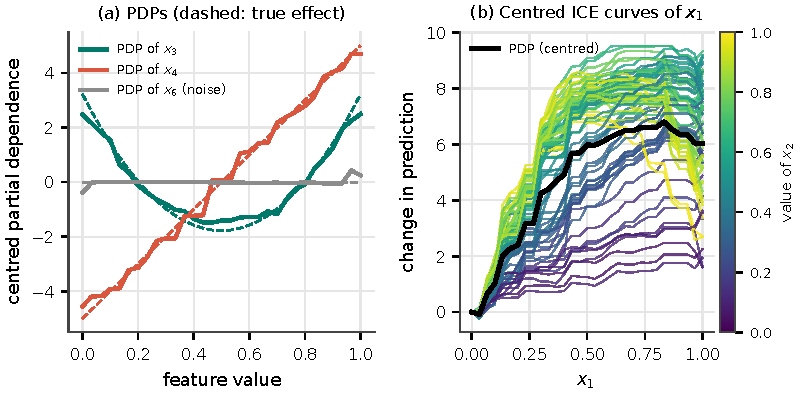
\includegraphics[width=\textwidth]{ch03/pdp_ice}
\caption{(a) Partial dependence plots of three features of a gradient boosting model of the
Friedman function, with the true effects dashed. (b) Centred ICE curves of $x_1$ for 80 instances,
coloured by their value of $x_2$; the thick line is the centred PDP.}
\label{fig:pdpice}
\end{figure}

PDPs are intuitive and easy to implement. Their main limitation is the assumption that the features
in $x_S$ are independent of those in $x_C$: if they are correlated, the average includes combinations
that are unlikely or impossible (a person 2 metres tall weighing 50 kg). Accumulated local effects\index{accumulated local effects}
(ALE) plots address this problem by averaging over the conditional distribution in small intervals
\citep{apley2020visualizing}. PDPs can display at most two features at once, should show the
distribution of the feature (they are unreliable where there are few data), and can hide
heterogeneous effects: if a feature increases the prediction for half of the data and decreases it
for the other half, the PDP is a flat line.

\subsection{Individual conditional expectation}

\emph{Individual conditional expectation\index{individual conditional expectation|textbf}} (ICE) plots draw one line per instance, showing how its
prediction changes when the feature changes and everything else stays fixed \citep{goldstein2015peeking};
the PDP is the average of the ICE lines. ICE plots reveal heterogeneous effects and interactions.
Because the lines start at different heights, it is useful to \emph{centre} them at a reference value
of the feature (for instance, its minimum) and plot only the change in prediction.
\Cref{fig:pdpice}b shows centred ICE curves of $x_1$: their slopes depend strongly on $x_2$ (yellow
lines, with high $x_2$, rise much more), which reveals the interaction $\sin(\pi x_1x_2)$ hidden in the
average. ICE plots are even more intuitive than PDPs, but they can display only one feature, become
overcrowded (use transparency or a sample of lines), and share the problem of unrealistic points with
correlated features.

\subsection{Feature interaction}

Two features \emph{interact} when the effect of one depends on the value of the other, that is, when
the prediction is not the sum of their individual effects. For instance, a model of house prices
without interaction might add 100,000 euros for a big house and 50,000 for a good location to a base
of 150,000; with an interaction, a big house in a good location would be worth an extra amount on top
of those two effects. Friedman's \emph{H-statistic\index{H-statistic@$H$-statistic|textbf}} \citep{friedman2008predictive} measures the share of
the variance of the joint partial dependence\index{partial dependence plot} that is due to the interaction. If two features $x_j$
and $x_k$ do not interact, their (centred) partial dependence decomposes as
$PD_{jk}(x_j,x_k)=PD_j(x_j)+PD_k(x_k)$, and
\begin{equation}
  H^2_{jk}=\frac{\sum_{i=1}^{n}\bigl[PD_{jk}(x_j^{(i)},x_k^{(i)})-PD_j(x_j^{(i)})-PD_k(x_k^{(i)})\bigr]^2}
                {\sum_{i=1}^{n}PD_{jk}^2(x_j^{(i)},x_k^{(i)})}.
\end{equation}
Similarly, the interaction of $x_j$ with all the other features compares the prediction with
$PD_j(x_j)+PD_{-j}(x_{-j})$. The statistic is dimensionless and, under an orthogonal decomposition (for instance with independent
features), a fraction between 0 (no interaction) and 1 (the
effect is pure interaction), and has a theory behind it, but it is expensive to compute (the cost
grows with the square of the number of instances, which is why it is estimated on a sample, adding
variance to the estimate), it is unclear when an interaction is significantly larger than zero, and it
does not show the shape of the interaction (a two-feature PDP does). With dependent features or estimated partial dependences it can exceed 1, and it is
undefined when the denominator vanishes, so the sampling scheme and the support of the data must be
checked before interpreting it. \Cref{lst:pdph} and
\cref{fig:importanceh}b find the only interaction of \cref{eq:friedman}: $H^2_{12}=0.083$, while the other
pairs are around 0.002.

\begin{pylisting}[label={lst:pdph}]{Partial dependence and Friedman's H statistic computed from scratch}
import numpy as np
from sklearn.datasets import make_friedman1
from sklearn.ensemble import GradientBoostingRegressor
from sklearn.model_selection import train_test_split

X, y = make_friedman1(n_samples=2000, n_features=10, noise=1.0, random_state=0)
X_tr, X_te, y_tr, y_te = train_test_split(X, y, test_size=0.3, random_state=0)
model = GradientBoostingRegressor(n_estimators=400, max_depth=3, learning_rate=0.05,
                                  random_state=0).fit(X_tr, y_tr)

def pd_at(X, cols, values):
    """Partial dependence: average prediction with the columns `cols` set to `values`."""
    Xv = X.copy()
    Xv[:, cols] = values
    return model.predict(Xv).mean()

def h2(X, j, k):
    """Friedman's H^2 for features j and k, from centred partial dependence functions."""
    pd = lambda cols: np.array([pd_at(X, cols, x[cols]) for x in X])
    pj, pk, pjk = pd([j]), pd([k]), pd([j, k])
    pj, pk, pjk = pj - pj.mean(), pk - pk.mean(), pjk - pjk.mean()
    return np.sum((pjk - pj - pk) ** 2) / np.sum(pjk ** 2)

S = X_te[:120]
print("PD of x4 at 0, 0.5, 1:", " ".join(f"{pd_at(S, [3], v):.2f}" for v in (0, 0.5, 1)))
for j, k in [(0, 1), (0, 3), (3, 4)]:
    print(f"H^2(x{j + 1}, x{k + 1}) = {h2(S, j, k):.3f}")
\end{pylisting}
\begin{pyoutput}
PD of x4 at 0, 0.5, 1: 9.77 14.44 19.00
H^2(x1, x2) = 0.083
H^2(x1, x4) = 0.002
H^2(x4, x5) = 0.002
\end{pyoutput}

\subsection{Permutation feature importance}

The importance of a feature can be measured by the increase of the prediction error of the model
after \emph{permuting} the values of that feature, which breaks its relationship with the target
\citep{breiman2001random,fisher2019all}: a feature is important if the model relied on it. The
algorithm is:
\begin{enumerate}
  \item compute the error $e_{\text{orig}}$ of the trained model (for example, the MSE\index{mean squared error (MSE)} or $1-\mathrm{AUC}$);
  \item for each feature $j$, permute its column in the data, compute the error $e_{\text{perm},j}$,
        and define the importance as the ratio $e_{\text{perm},j}/e_{\text{orig}}$ or the difference
        $e_{\text{perm},j}-e_{\text{orig}}$ (repeating the permutation to reduce the variance);
  \item sort the features by importance.
\end{enumerate}
Its interpretation is clear (the loss of performance when the information of the feature is
destroyed), it gives a compressed global view of the model, and the ratio version is comparable
across problems. It needs the true target (it cannot be computed with only a model and unlabelled
data), it is tied to the error of the model, which is not what we want if the question is how much of
the output varies with each feature, and it should be computed on \emph{test} data, since importance
on training data reflects what the model memorised. With correlated features, permuting one creates
unrealistic instances and the importance is shared between the correlated features.

\begin{pylisting}[label={lst:importance}]{Permutation importance, impurity importance and global surrogates}
import numpy as np
from sklearn.datasets import make_friedman1
from sklearn.ensemble import RandomForestRegressor
from sklearn.inspection import permutation_importance
from sklearn.metrics import r2_score
from sklearn.model_selection import train_test_split
from sklearn.tree import DecisionTreeRegressor

X, y = make_friedman1(n_samples=2000, n_features=10, noise=1.0, random_state=0)
X_tr, X_te, y_tr, y_te = train_test_split(X, y, test_size=0.3, random_state=0)
rf = RandomForestRegressor(300, random_state=0).fit(X_tr, y_tr)
pi = permutation_importance(rf, X_te, y_te, n_repeats=10, random_state=0)   # drop in R^2
for j in np.argsort(-pi.importances_mean)[:6]:
    print(f"x{j + 1:<2d} permutation={pi.importances_mean[j]:.3f} "
          f"+/- {pi.importances_std[j]:.3f}   impurity={rf.feature_importances_[j]:.3f}")
for depth in (2, 3, 5):        # global surrogate: a small tree that imitates the forest
    tree = DecisionTreeRegressor(max_depth=depth, random_state=0)
    tree.fit(X_tr, rf.predict(X_tr))
    print(f"surrogate tree of depth {depth}: R^2 with respect to the forest = "
          f"{r2_score(rf.predict(X_te), tree.predict(X_te)):.3f}")
\end{pylisting}
\begin{pyoutput}
x4  permutation=0.714 +/- 0.032   impurity=0.367
x1  permutation=0.437 +/- 0.021   impurity=0.208
x2  permutation=0.386 +/- 0.036   impurity=0.216
x5  permutation=0.138 +/- 0.012   impurity=0.097
x3  permutation=0.077 +/- 0.005   impurity=0.057
x7  permutation=0.000 +/- 0.000   impurity=0.012
surrogate tree of depth 2: R^2 with respect to the forest = 0.510
surrogate tree of depth 3: R^2 with respect to the forest = 0.747
surrogate tree of depth 5: R^2 with respect to the forest = 0.877
\end{pyoutput}

\Cref{lst:importance} and \cref{fig:importanceh}a compare permutation importance\index{feature importance!permutation} on test data with the
impurity-based\index{feature importance} importance of a random forest (\cref{sec:enspractice}). Both rank $x_4$, $x_1$, $x_2$,
$x_5$ and $x_3$ first, but the impurity importance gives every noise feature around 0.01, whereas their
permutation importance is zero: the forest used them to fit noise in the training data, and that does
not help on new data.

\begin{figure}[htbp]
\centering
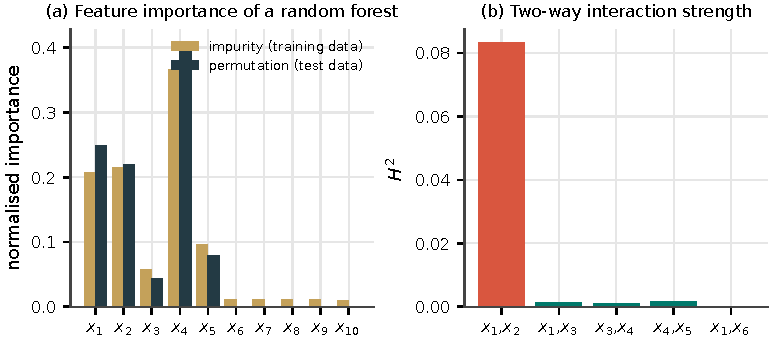
\includegraphics[width=\textwidth]{ch03/importance_h}
\caption{(a) Normalised impurity-based and permutation importance of a random forest fitted to the
Friedman function ($x_6$ to $x_{10}$ are noise). (b) $H^2$ interaction strength for five pairs of
features of the gradient boosting model.}
\label{fig:importanceh}
\end{figure}

\subsection{Global surrogate models}

A \emph{global surrogate\index{global surrogate|textbf}} is an interpretable model trained to approximate the predictions of a
black box; it is the mimetic\index{mimetic classifier} classifier of \cref{sec:drawbacks}, under another name (it is also known
as approximation model, metamodel, response surface model or emulator). The procedure is to choose a
data set, obtain the predictions $\hat y$ of the black box on it, train an interpretable model
(linear, tree\dots) on those predictions, and measure how well it replicates them, for instance with
\begin{equation}
  R^2=1-\frac{\sum_i(\hat y_*^{(i)}-\hat y^{(i)})^2}{\sum_i(\hat y^{(i)}-\bar{\hat y})^2},
\end{equation}
where $\hat y_*$ are the predictions of the surrogate. Only then is the surrogate interpreted. In
\cref{lst:importance}, a tree of depth 2 captures 51\% of the variance of the forest's predictions,
depth 3 captures 75\% and depth 5 captures 88\%.

The method is flexible, intuitive, and its fidelity\index{fidelity} is easy to measure, but several cautions apply.
It draws conclusions about the model, not about the data. There is no clear cut-off for a good
enough $R^2$, and the surrogate may be very close to the black box in some regions and far from it in
others. If the input distribution is changed, for instance by weighting the instances around a
particular point, the surrogate becomes \emph{local}, which leads to LIME\index{LIME}.

\subsection{Local surrogates: LIME}

LIME\index{LIME} (local interpretable model-agnostic explanations, \citealp{ribeiro2016should}) was introduced in
\cref{sec:drawbacks}. To explain the prediction of a black box $f$ for an instance $x$, it
\begin{enumerate}
  \item generates a data set of perturbed instances and obtains the black box predictions for them;
  \item weights the new samples by their proximity to $x$, with a kernel $\pi_x$;
  \item fits a weighted interpretable model (a Lasso, a short tree) with a small number $K$ of features;
  \item explains the prediction by interpreting the local model.
\end{enumerate}
The local model must be faithful\index{faithfulness} in the neighbourhood of $x$ (\emph{local fidelity\index{fidelity|textbf}}), not globally.
How the perturbations are generated depends on the data: for text, LIME removes words at random and
represents each variant by the presence or absence of each word; for images, it switches off
\emph{superpixels} (groups of similar neighbouring pixels), replacing them by grey; for tabular data,
it draws each feature from a normal distribution with the mean and standard deviation of the training
data, so the samples come from the centre of the data and not from around $x$, and the kernel decides
which of them matter.

\begin{pylisting}[label={lst:lime}]{A minimal implementation of LIME for tabular data}
import numpy as np
from sklearn.ensemble import GradientBoostingRegressor
from sklearn.linear_model import Ridge
from apartments import FEATURES, apartments

def lime(f, X_train, x, n=5000, kernel_width=None, seed=0):
    """LIME for tabular data: a weighted linear model fitted to perturbed samples."""
    rng = np.random.default_rng(seed)
    mu, sd = X_train.mean(axis=0), X_train.std(axis=0)
    # samples from the data distribution
    Z = rng.normal(mu, sd, (n, len(x)))
    d = np.linalg.norm((Z - x) / sd, axis=1)              # standardised distance to x
    width = kernel_width or 0.75 * np.sqrt(len(x))
    w = np.exp(-d ** 2 / width ** 2)                      # proximity weights
    g = Ridge(alpha=1.0).fit((Z - mu) / sd, f(Z), sample_weight=w)
    return g.coef_, g.score((Z - mu) / sd, f(Z), sample_weight=w)

X, y = apartments()
model = GradientBoostingRegressor(random_state=0).fit(X, y)
x = np.array([1.0, 0.0, 50.0, 2.0])         # park nearby, cat forbidden, 50 m2, 2nd floor
for seed, width in [(0, None), (1, None), (2, None), (0, 0.5)]:
    coef, fid = lime(model.predict, X, x, kernel_width=width, seed=seed)
    print(f"seed {seed}, width {width or 1.5:.1f}: "
          + " ".join(f"{n}={c:.1f}" for n, c in zip(FEATURES, coef)) + f"  R2={fid:.2f}")
\end{pylisting}
\begin{pyoutput}
seed 0, width 1.5: park_nearby=8.8 cat_allowed=6.4 area_m2=71.3 floor=6.3  R2=0.97
seed 1, width 1.5: park_nearby=9.0 cat_allowed=6.4 area_m2=70.6 floor=5.6  R2=0.97
seed 2, width 1.5: park_nearby=8.7 cat_allowed=7.1 area_m2=71.4 floor=5.5  R2=0.97
seed 0, width 0.5: park_nearby=0.3 cat_allowed=0.7 area_m2=42.5 floor=-0.4  R2=0.80
\end{pyoutput}

\Cref{lst:lime} implements LIME and explains the price predicted by a gradient boosting\index{gradient boosting} model for a
flat of 50 square metres, on the second floor, near a park and in a building where cats are forbidden
(the synthetic apartment data of \cref{lst:apartments}). With the default kernel width the
explanation is stable across random seeds and faithful ($R^2=0.97$): the area dominates (71 thousand
euros per standard deviation), followed by the park (about 9). With a narrower kernel the explanation
changes completely (only the area matters, with half the weight) and is less faithful ($R^2=0.80$). Part of this change is not about locality: with unnormalised weights and a
fixed Ridge penalty, a narrower kernel also increases the relative regularisation, and the Gaussian
perturbations produce invalid inputs, such as fractional values of the binary features. A careful
implementation samples valid inputs, normalises the weights, reports the effective sample size\index{sample size}\index{effective sample size} and
measures fidelity on fresh perturbations.
This is LIME's main problem: the definition of the neighbourhood is an open question, there is no
principled way of choosing the kernel width, the Gaussian sampling ignores correlations between
features, and the explanations can be unstable \citep{alvarezmelis2018robustness}. They can also be
manipulated: a model can be built to behave in a biased way on real data and innocuously on the
perturbed samples that LIME generates \citep{slack2020fooling}. On the positive side, LIME works for
tabular data, text and images, its explanations are short and possibly contrastive, it gives a
fidelity measure, and it can use interpretable features different from those of the model.

\subsection{Shapley values}

The \emph{Shapley\index{Shapley values|textbf} value} comes from cooperative game theory \citep{shapley1953value}. It distributes the
payout of a game fairly among the players that cooperated to obtain it. To explain a prediction
\citep{strumbelj2014explaining}, the game is the prediction task for one instance, the players are its
feature values, and the payout is the prediction minus the average prediction. The value of a
coalition $S$ of features is the expected prediction when the features in $S$ are fixed to the values
of the instance and the others are drawn from the data,
$v(S)=\E\bigl[\hat f(x_S,X_{\bar S})\bigr]-\E[\hat f(X)]$, and the Shapley value of feature $j$ is its
average marginal contribution over all the coalitions:
\begin{equation}\label{eq:shapley}
  \phi_j=\sum_{S\subseteq F\setminus\{j\}}\frac{|S|!\,(p-|S|-1)!}{p!}\,\bigl(v(S\cup\{j\})-v(S)\bigr),
\end{equation}
where $F$ is the set of $p$ features. The weights correspond to averaging over all the orders in which
the features could join the coalition. The Shapley value is the only attribution that satisfies four
properties: \emph{efficiency} (the contributions add up to the difference between the prediction and
the average, $\sum_j\phi_j=\hat f(x)-\E[\hat f(X)]$), \emph{symmetry} (two features that contribute
equally to every coalition get the same value), \emph{dummy} (a feature that never changes the
prediction gets zero) and \emph{additivity} (for a sum of models, the values add).

\begin{pylisting}[label={lst:apartments}]{Synthetic apartment prices used in the explanation examples}
"""Synthetic apartment prices used in the explanation examples (Unit 3)."""
import numpy as np

FEATURES = ["park_nearby", "cat_allowed", "area_m2", "floor"]

def apartments(n=2000, seed=0):
    rng = np.random.default_rng(seed)
    area = rng.uniform(30, 120, n)
    park = (rng.random(n) < 0.5).astype(float)
    cat = (rng.random(n) < 0.6).astype(float)
    floor = rng.integers(0, 8, n).astype(float)
    price = (40 + 2.6 * area + 25 * park + 15 * cat + 3 * floor     # thousand EUR
             + 0.3 * park * (area - 75) + rng.normal(0, 12, n))
    return np.c_[park, cat, area, floor], price
\end{pylisting}

\begin{pylisting}[label={lst:shapley}]{Exact Shapley values by enumerating all coalitions}
from itertools import combinations
from math import factorial
import numpy as np
from sklearn.ensemble import GradientBoostingRegressor
from apartments import FEATURES, apartments

def shapley(f, x, background):
    """Exact Shapley values; absent features take their values from background data."""
    p = len(x)
    def value(S):                                   # v(S) = E[f(x_S, X_rest)]
        Z = background.copy()
        Z[:, list(S)] = x[list(S)]
        return f(Z).mean()
    phi = np.zeros(p)
    for j in range(p):
        others = [k for k in range(p) if k != j]
        for size in range(p):
            for S in combinations(others, size):
                weight = factorial(size) * factorial(p - size - 1) / factorial(p)
                phi[j] += weight * (value(S + (j,)) - value(S))
    return phi

X, y = apartments()
model = GradientBoostingRegressor(random_state=0).fit(X, y)
x = np.array([1.0, 0.0, 50.0, 2.0])
bg = X[np.random.default_rng(1).choice(len(X), 300, replace=False)]
phi = shapley(model.predict, x, bg)
base, pred = model.predict(bg).mean(), model.predict(x[None])[0]
for name, v in zip(FEATURES, phi):
    print(f"{name:12s} {v:+7.1f}")
print(f"average {base:.1f} + contributions {phi.sum():+.1f} = {base + phi.sum():.1f}"
      f"   (prediction {pred:.1f})")
\end{pylisting}
\begin{pyoutput}
park_nearby     +9.4
cat_allowed     -8.3
area_m2        -70.3
floor           -4.6
average 264.7 + contributions -73.9 = 190.8   (prediction 190.8)
\end{pyoutput}

\Cref{lst:shapley} computes the exact values for the flat explained with LIME\index{LIME}, enumerating the
$2^3$ coalitions of the other features for each of the four features and estimating $v(S)$ with 300
background flats. The average predicted price is 264.7 thousand euros and this flat's prediction is
190.8: being small (50 square metres) lowers the price by 70.3, the forbidden cats by 8.3 and the floor
by 4.6, while the park raises it by 9.4, and the contributions add up exactly to the difference of
$-73.9$ (\cref{fig:limeshap}a).

\begin{figure}[htbp]
\centering
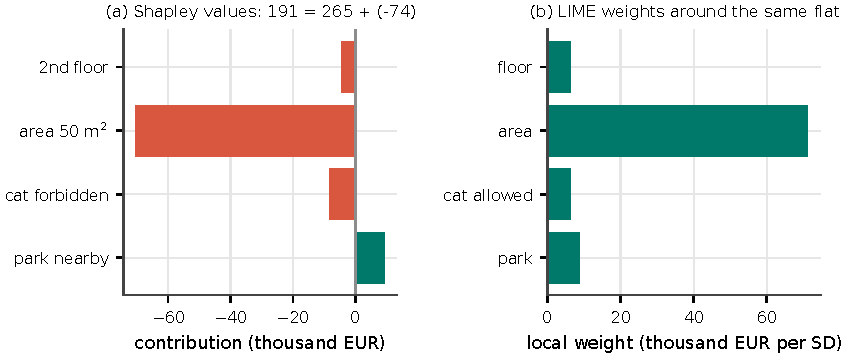
\includegraphics[width=\textwidth]{ch03/lime_shap}
\caption{Two explanations of the predicted price of one flat. (a) Shapley values: contributions to the
difference between the prediction and the average prediction. (b) LIME: weights of a local linear
model, per standard deviation of each feature.}
\label{fig:limeshap}
\end{figure}

Comparing the two panels of \cref{fig:limeshap} shows that the two methods answer different
questions. LIME's weights are local \emph{slopes}: around this flat, more area means a higher price
(+71 per standard deviation), and allowing cats would raise it. Shapley values are
\emph{contributions} relative to the average flat: this flat's area, smaller than average, lowers its
price by 70, and its cat ban lowers it by 8. Neither is ``the'' explanation.

For a fixed cooperative game, the Shapley value is the unique allocation that satisfies its classical
axioms (other attribution methods, such as integrated gradients\index{integrated gradients}, have axiomatic foundations of their
own \citep{sundararajan2017axiomatic}); it distributes the difference among the features according to
those axioms, and it allows contrastive explanations (against the average, or
against a subset of instances). But it is expensive: the number of coalitions grows exponentially with
the number of features, so in practice it is approximated by sampling coalitions and background
instances \citep{strumbelj2014explaining} or computed with model-specific algorithms, as in the SHAP\index{SHAP}
library \citep{lundberg2017unified}. It is also easy to misinterpret: the Shapley value of a feature is
\emph{not} the difference in prediction if the feature were removed from the model, and it does not
support statements such as ``if I earned 300 euros more, my score would go up by 5 points'', because it
returns one value per feature, not a model. It uses all the features, so it is the wrong method if
sparse explanations are wanted, and, like the PDP, it evaluates the model on unrealistic combinations
when features are correlated.

% ---------------------------------------------------------------------
\section{Example-based explanations}\label{sec:examplebased}

Example-based methods explain a model, or the data it was trained on, by selecting particular
instances instead of summarising features. People reason this way all the time: a physician who
sees a patient with an unusual cough remembers a similar case; a data scientist starting a project
reuses the code of a similar one; a firefighter decides not to enter a burning house because a
similar one collapsed. These methods are mostly model-agnostic, but they only make sense if an
instance can be presented in a way people understand, as with images or text; they work poorly for
tabular data with hundreds of features. We consider four kinds: counterfactual instances, adversarial
examples\index{adversarial example}, prototypes\index{prototypes and criticisms} and criticisms, and influential instances\index{influential instance} ($k$-nearest neighbours\index{k-nearest neighbours@$k$-nearest neighbours}, the fifth,
was discussed in \cref{sec:intmodels}).

\subsection{Counterfactual explanations}

A counterfactual explanation\index{counterfactual explanation} describes a causal situation of the form ``if $X$ had not occurred, $Y$
would not have occurred''. For a prediction, the ``event'' is the predicted outcome and the ``causes''
are the feature values of the instance: even if the relation between inputs and outcome is not causal
in the world, it is causal \emph{for the model}. A counterfactual explanation of a prediction
describes \emph{the smallest change to the feature values that changes the prediction to a
predefined output}. Peter applies for a loan and is rejected: what is the smallest change to his
income or debts that would get him the loan? Anna's model predicts that her flat can be rented for
900 euros, but she expected 1000: what would make it worth 1000?

Counterfactuals are human-friendly explanations: they are contrastive and selective. A good
counterfactual should produce the desired prediction as closely as possible, be as similar as possible
to the instance, change as few features as possible, and have likely feature values (we cannot suggest
a flat with a negative size). It should also be \emph{actionable}: changing one's age or past is not
possible, and recommending it is useless \citep{ustun2019actionable}. There are usually many
counterfactuals (a \emph{Rashomon} effect), which can be addressed by reporting several diverse ones
\citep{mothilal2020explaining} or by a criterion to choose the best.

\citet{wachter2018counterfactual} proposed to find a counterfactual $x'$ for the instance $x$ and the
desired outcome $y'$ by minimising
\begin{equation}
  L(x,x',y',\lambda)=\lambda\,\bigl(\hat f(x')-y'\bigr)^2+d(x,x'),
\end{equation}
where the first term pushes the prediction towards $y'$ and the second keeps $x'$ close to $x$, with the
Manhattan distance weighted by the inverse \emph{median absolute deviation} of each feature,
\begin{equation}
  d(x,x')=\sum_{j=1}^{p}\frac{|x_j-x'_j|}{\mathrm{MAD}_j},\qquad
  \mathrm{MAD}_j=\operatorname{median}_{i}\bigl|x_{ij}-\operatorname{median}_l x_{lj}\bigr| .
\end{equation}
This distance is robust to outliers and, being an $L_1$ distance, prefers changing few features. The
algorithm starts with a small $\lambda$ and increases it until the prediction of the minimiser is
within a tolerance $\epsilon$ of $y'$, so that among the solutions that achieve the outcome it returns a
close one. The method needs no access to the data or to the internals of the model, works even for
systems that do not use machine learning, and is easy to implement; but there is no guarantee of
finding a counterfactual within the tolerance, and categorical features with many levels make the search
expensive.

\begin{pylisting}[label={lst:counterfactual}]{A counterfactual explanation with the method of Wachter et al.}
import numpy as np
from scipy.optimize import minimize
from sklearn.linear_model import LogisticRegression
from loans import FEATURES, loan_data

X, y = loan_data()
model = LogisticRegression(C=1e6, max_iter=5000).fit(X, y)
f = lambda Z: model.predict_proba(Z)[:, 1]                    # P(repay)
mad = np.median(np.abs(X - np.median(X, axis=0)), axis=0)      # median absolute deviation
lo, hi = X.min(axis=0), X.max(axis=0)                          # plausible ranges

def counterfactual(x, target=0.5, free=(0, 1), lambdas=(1, 10, 100, 1000, 10000), tol=0.01):
    """Wachter et al.: minimise lam*(f(x')-target)^2 + MAD-weighted L1 distance to x."""
    free = list(free)
    def loss(z, lam):
        xc = x.copy()
        xc[free] = z
        out = np.sum(np.maximum(lo - xc, 0) + np.maximum(xc - hi, 0))   # stay plausible
        dist = np.sum(np.abs(xc - x)[free] / mad[free])          # MAD-weighted L1 distance
        return lam * (f(xc[None])[0] - target) ** 2 + dist + 1e3 * out
    z = x[free].copy()
    for lam in lambdas:                                        # raise lambda until close
        z = minimize(loss, z, args=(lam,), method="Nelder-Mead").x
        xc = x.copy()
        xc[free] = z
        if abs(f(xc[None])[0] - target) <= tol:
            break
    return xc

peter = np.array([30.0, 0.45, 5.0, 0.0])     # income, debt ratio, years in job, no default
# only income and debt ratio may change; aim just above the bank's threshold of 0.5
cf = counterfactual(peter, target=0.51, tol=0.005)
print(f"Peter:          P(repay) = {f(peter[None])[0]:.3f}")
print(f"counterfactual: P(repay) = {f(cf[None])[0]:.3f}")
print("decision:", "approved" if f(cf[None])[0] >= 0.5 else "still rejected")
for name, a, b in zip(FEATURES, peter, cf):
    if abs(a - b) > 1e-3:
        print(f"  {name}: {a:.3f} -> {b:.3f}")
\end{pylisting}
\begin{pyoutput}
Peter:          P(repay) = 0.289
counterfactual: P(repay) = 0.507
decision: approved
  debt_ratio: 0.450 -> 0.139
\end{pyoutput}

\Cref{lst:counterfactual} and \cref{fig:counterfactual} find a counterfactual for Peter with the
logistic regression of \cref{lst:odds}, allowing only his income and debt ratio to change and keeping
them within the range of the data. His probability of repaying is 0.289; reducing his debt ratio from
0.45 to 0.14 raises it to 0.507, just above the bank's threshold of 0.5. The search aims slightly above
the threshold and the listing checks the decision: a counterfactual is valid only if it obtains the
desired decision, and accepting any point within a tolerance on either side of 0.5 could leave Peter
still rejected. The $L_1$ distance produced a sparse answer: it
was cheaper, in units of median absolute deviation, to reduce the debt than to increase the income.

\begin{figure}[htbp]
\centering
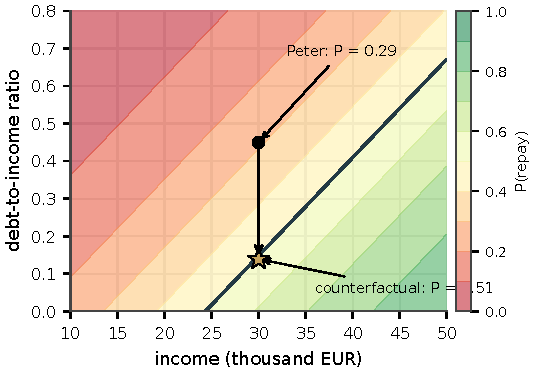
\includegraphics[width=0.66\textwidth]{ch03/counterfactual}
\caption{A counterfactual explanation for a rejected loan application. The colours show the predicted
probability of repayment as a function of income and debt ratio (other features fixed); the line is the
acceptance boundary.}
\label{fig:counterfactual}
\end{figure}

\subsection{Adversarial examples}

An \emph{adversarial example\index{adversarial example|textbf}} is an instance with small, intentional perturbations that make a model
give a false prediction: a counterfactual whose aim is to deceive the model rather than to explain it.
A stop sign with a few stickers that a car's vision system reads as a speed limit sign
\citep{eykholt2018robust}, or a spam message disguised as a normal one, are examples. Most methods
minimise the distance between the adversarial example and the original while pushing the prediction
towards the desired (wrong) output. Some need the gradients of the model, others only its predictions:
\begin{itemize}
  \item the \emph{fast gradient sign\index{fast gradient sign method (FGSM)|textbf} method} \citep{goodfellow2015explaining} moves every input feature
        by a small step $\epsilon$ in the direction that increases the loss $J$ of the true class,
        \begin{equation}\label{eq:fgsm}
          x'=x+\epsilon\cdot\operatorname{sign}\bigl(\nabla_xJ(\theta,x,y)\bigr);
        \end{equation}
        many tiny changes add up to a large change in the output, which works because many models behave
        almost linearly in high-dimensional spaces;
  \item the \emph{one-pixel attack} \citep{su2019one} changes a single pixel, found with differential
        evolution: a population of candidate modifications (coordinates and colour) evolves until one of
        them fools the classifier;
  \item the \emph{adversarial patch} \citep{brown2017adversarial} drops the requirement of a small
        perturbation and optimises a printable sticker that makes any object look, for instance, like a
        toaster to the classifier, across different backgrounds and positions;
  \item \emph{robust} adversarial examples work in the physical world under changes of viewpoint,
        lighting or noise; the \emph{expectation over transformation} method \citep{athalye2018synthesizing}
        maximises the expected probability of the target class over a distribution $T$ of
        transformations, keeping the expected distance to the original below a threshold, and was used to
        3D-print a turtle that a neural network classified as a rifle from almost every angle;
  \item \emph{black-box attacks} \citep{papernot2017practical} need neither the model nor the training
        data: the attacker queries the model, trains a surrogate\index{global surrogate} (a mimetic\index{mimetic classifier} model, \cref{sec:drawbacks}),
        crafts adversarial examples for the surrogate, and uses them against the original, exploiting the
        fact that adversarial examples \emph{transfer} between models.
\end{itemize}
We study adversarial examples as a security threat, with an experiment, in \cref{sec:adversarial}.
From the interpretability point of view, understanding which features matter and how they affect the
prediction is a proactive step towards finding the weaknesses of a model.

\subsection{Prototypes and criticisms}

A \emph{prototype\index{prototypes and criticisms|textbf}} is a data instance that is representative of the data; a \emph{criticism} is an
instance that is not well represented by the set of prototypes. Prototypes summarise complex
distributions, and criticisms point at what the summary misses. Both are real instances.
MMD-critic\index{MMD-critic} \citep{kim2016examples} selects them by comparing distributions with the \emph{maximum mean
discrepancy} \citep{gretton2012kernel}. For prototypes $z_1,\dots,z_m$ and data $x_1,\dots,x_n$,
\begin{equation}
  \mathrm{MMD}^2=\frac{1}{m^2}\sum_{i,j=1}^{m}k(z_i,z_j)-\frac{2}{mn}\sum_{i=1}^{m}\sum_{j=1}^{n}k(z_i,x_j)
                +\frac{1}{n^2}\sum_{i,j=1}^{n}k(x_i,x_j),
\end{equation}
where $k$ is a kernel that measures the similarity\index{similarity measure} of two points, for instance the radial basis
function $k(x,x')=e^{-\gamma\|x-x'\|^2}$. The closer $\mathrm{MMD}^2$ is to zero, the better the
prototypes represent the data. Prototypes are selected greedily: starting with an empty list, add at each
step the instance that most reduces $\mathrm{MMD}^2$. Criticisms are found with the \emph{witness
function}, which estimates how much the two densities differ at a point $x$,
\begin{equation}
  \mathrm{witness}(x)=\frac1n\sum_{i=1}^{n}k(x,x_i)-\frac1m\sum_{j=1}^{m}k(x,z_j):
\end{equation}
positive values mark regions where the data are under-represented by the prototypes, negative values
regions where they are over-represented. Criticisms are the instances with extreme witness values, also
selected greedily (in practice with a term that keeps them diverse).

\begin{pylisting}[label={lst:mmdcritic}]{Greedy selection of prototypes and criticisms with MMD-critic}
import numpy as np

def rbf(A, B, gamma):
    return np.exp(-gamma * ((A[:, None, :] - B[None, :, :]) ** 2).sum(-1))

def mmd_critic(X, m, c, gamma=0.5, radius=1.0):
    """MMD-critic (Kim et al., 2016): greedy prototypes and criticisms."""
    K = rbf(X, X, gamma)
    # mean similarity of each point to the data
    colmean = K.mean(axis=0)
    protos, path = [], []
    for _ in range(m):
        cands = [i for i in range(len(X)) if i not in protos]
        sets = [protos + [i] for i in cands]               # candidate prototype sets
        score = [K[np.ix_(s, s)].mean() - 2 * colmean[s].mean() for s in sets]
        protos.append(cands[int(np.argmin(score))])
        path.append(min(score) + K.mean())      # add the constant mean k(x,x')
    witness = colmean - K[:, protos].mean(axis=1)
    crit = []                          # most under-represented points, `radius` apart
    for i in np.argsort(-witness):
        if i not in protos and all(np.linalg.norm(X[i] - X[j]) > radius for j in crit):
            crit.append(i)
        if len(crit) == c:
            break
    return protos, crit, path, witness

rng = np.random.default_rng(5)
X = np.vstack([rng.normal([0, 0], 0.5, (240, 2)), rng.normal([3, 0.5], 0.6, (160, 2)),
               rng.normal([1.5, 3], 0.45, (90, 2)), rng.normal([4.2, 3.4], 0.25, (25, 2))])
protos, crit, path, witness = mmd_critic(X, m=4, c=3)
print("MMD^2 as prototypes are added:", np.round(path, 4))
print("prototypes:", np.round(X[protos], 1).tolist())
print("criticisms:", np.round(X[crit], 1).tolist())
print("their witness values:", np.round(witness[crit], 3))
\end{pylisting}
\begin{pyoutput}
MMD^2 as prototypes are added: [0.4701 0.125  0.062  0.0377]
prototypes: [[0.1, -0.0], [2.9, 0.6], [1.6, 3.0], [-0.3, 0.0]]
criticisms: [[4.2, 3.4], [2.0, -0.7], [3.9, -0.4]]
their witness values: [0.05  0.034 0.034]
\end{pyoutput}

In \cref{lst:mmdcritic} and \cref{fig:mmd}, four prototypes reduce $\mathrm{MMD}^2$ from 0.47 to 0.04:
two in the largest group and one in each of the other two. The criticisms are the small group of 25
instances at the top right, which no prototype represents, and two instances at the edges of the
groups. MMD-critic helps to understand a data distribution, to build interpretable models such as a
\emph{nearest prototype classifier} (which predicts the class of the closest prototype and returns it as
the explanation), and to audit a black box: predict the prototypes and criticisms, and look at the cases
where the model is wrong. In experiments with people, sets of prototypes and criticisms helped
participants understand a classification better than random examples. The drawbacks are that the
numbers of prototypes and criticisms must be chosen (a plot of $\mathrm{MMD}^2$ against the number of
prototypes helps), as must the kernel and its scale, and that all features are used, relevant or not.

\begin{figure}[htbp]
\centering
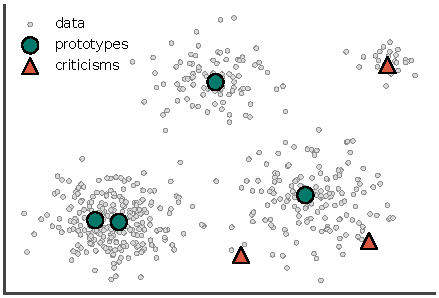
\includegraphics[width=0.58\textwidth]{ch03/mmd_critic}
\caption{Prototypes and criticisms selected by MMD-critic on a two-dimensional data set.}
\label{fig:mmd}
\end{figure}

\subsection{Influential instances}

A training instance is \emph{influential\index{influential instance|textbf}} if deleting it considerably changes the parameters or the
predictions of the model. With influential instances we do not treat the model as fixed but as a
function of the training data, which helps to debug it: we learn for which instances the model could
have problems, which training instances should be checked for errors, and how robust the model is. We
might not trust a model whose parameters depend strongly on a single instance.

An influential instance is not the same as an \emph{outlier}, an instance far from the others: an
outlier is influential only if it changes the model, which also depends on its target value.
\emph{Deletion diagnostics\index{deletion diagnostics|textbf}} retrain the model without each instance $i$ and measure the change:
\begin{equation}
  \mathrm{DFBETA}_i=\beta-\beta^{(-i)},\qquad
  D_i=\frac{\sum_{j=1}^{n}\bigl(\hat y_j-\hat y_j^{(-i)}\bigr)^2}{p\cdot\mathrm{MSE}},
\end{equation}
where $\beta^{(-i)}$ and $\hat y_j^{(-i)}$ are the parameters and predictions of the model trained without
instance $i$, and $D_i$ is \emph{Cook's distance\index{Cook's distance|textbf}} \citep{cook1977detection}, with $p$ parameters. DFBETA
needs a model with parameters; Cook's distance does not, but the MSE\index{mean squared error (MSE)} is not meaningful for every model,
and the simplest model-agnostic measure is the mean absolute change of the predictions. We can also
measure the influence of each training instance on the prediction for a particular instance, and model
the influence as a function of the features (for instance, with a short tree) to find out what kind of
training instances are most influential.

\begin{pylisting}[label={lst:influence}]{Deletion diagnostics: DFBETA and Cook's distance}
import numpy as np
from sklearn.linear_model import LinearRegression

rng = np.random.default_rng(7)
x = np.r_[rng.uniform(0, 5, 30), 12.0]                  # last point: high leverage...
y = np.r_[2 * x[:30] + 1 + rng.normal(0, 1.2, 30), 6.0] # ...and off the trend
X = x[:, None]
full = LinearRegression().fit(X, y)
yhat = full.predict(X)
s2 = np.sum((y - yhat) ** 2) / (len(y) - 2)              # residual variance (2 parameters)
dfbeta, cook = [], []
for i in range(len(y)):                       # deletion diagnostics: refit without i
    m = LinearRegression().fit(np.delete(X, i, 0), np.delete(y, i))
    dfbeta.append(full.coef_[0] - m.coef_[0])
    cook.append(np.sum((yhat - m.predict(X)) ** 2) / (2 * s2))
for i in np.argsort(cook)[::-1][:3]:
    print(f"instance {i:2d}: x={x[i]:5.2f}  DFBETA={dfbeta[i]:+.3f}  "
          f"Cook's D={cook[i]:.3f}")
\end{pylisting}
\begin{pyoutput}
instance 30: x=12.00  DFBETA=-1.237  Cook's D=17.473
instance 19: x= 4.94  DFBETA=+0.078  Cook's D=0.140
instance 16: x= 4.98  DFBETA=+0.059  Cook's D=0.080
\end{pyoutput}

In \cref{lst:influence} and \cref{fig:influence}, a single instance with an extreme value of $x$ that
does not follow the trend changes the slope of a regression from 2.12 to 0.88; its Cook's distance is
17.5, while the next largest is 0.14.

\begin{figure}[htbp]
\centering
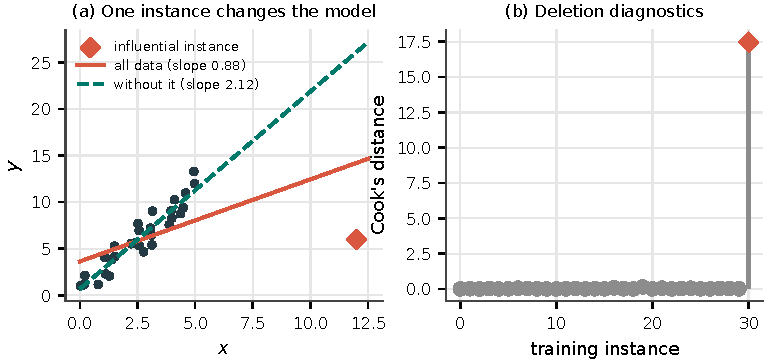
\includegraphics[width=\textwidth]{ch03/influence}
\caption{(a) A linear regression with and without one influential instance. (b) Cook's distance of each
training instance.}
\label{fig:influence}
\end{figure}

Deletion diagnostics are expensive, because the model must be retrained once per instance.
\emph{Influence functions\index{influence function|textbf}} \citep{koh2017understanding} approximate them for models with differentiable
losses: upweighting an instance $z$ by an infinitesimal $\epsilon$ changes the parameters by
approximately
\begin{equation}
  \hat\theta_{\epsilon,z}-\hat\theta\approx-\epsilon\,H_{\hat\theta}^{-1}\nabla_\theta L(z,\hat\theta),
\end{equation}
the gradient of the loss of $z$ scaled by the inverse Hessian $H_{\hat\theta}$ of the training loss (the
curvature). Here the training loss is the average $\frac1n\sum_iL(z_i,\theta)$ and $z$ receives the extra
weight $\epsilon$; removing $z$ corresponds to $\epsilon=-1/n$, which reverses the sign:
$\hat\theta_{-z}-\hat\theta\approx\frac1n H_{\hat\theta}^{-1}\nabla_\theta L(z,\hat\theta)$. The approximation
requires a regular optimum with an invertible Hessian. Influential instances are among the best debugging tools: they reveal the weaknesses of a
model, help to handle domain mismatch between training and test data (which training instances caused an
error?), tell us which training labels to check first when we cannot check them all, and can be compared
across models. Influence functions can even be used to create adversarial training\index{adversarial training} data. Their limits:
they only consider single instances, there is no clear cut-off for calling an instance influential, and
influence functions are an approximation, validated mostly empirically.

\subsection{The future of interpretability}

Interpretability tools catalyse the adoption of machine learning: since the goal of a model can never be
specified perfectly, interpretability is needed to close the gap between the specified and the actual
goal, and many organisations and industries demand transparency for legal reasons, for risk aversion or
to gain insight. The focus is moving towards model-agnostic tools, interpretability is being automated
along with model building (Unit~4), and systems are increasingly expected to explain themselves.
Regulation pushes in the same direction: the debate on whether the European data protection regulation
grants a ``right to explanation\index{right to explanation}'' of automated decisions \citep{goodman2017european,wachter2018counterfactual}
was followed by the European Artificial Intelligence Act \citep{eu2024aiact}, which imposes transparency,
documentation and human oversight requirements on high-risk\index{AI Act!high-risk systems} systems.

% =====================================================================
\section{Machine learning and security}\label{sec:security}

As soon as enough computers were connected, some people realised that the network was a perfect
medium to make money, often illegitimately. Spam is the classic example, and it shows both the
promise and the difficulty of using machine learning in security \citep{chio2018machine}. Machine
learning was not invented by spam fighters, but it was quickly adopted by those who saw its potential
against a constantly evolving source of abuse. Content-based\index{content-based filtering} models learned from e-mail data recognise
spam in a generalisable way; metadata and the reputation of senders add evidence; and a feedback loop
with users, who mark messages as spam, builds a collective intelligence that improves over time. Spam
filters have evolved to deal with an ever-growing diversity\index{diversity} of circumvention methods, and today the vast
majority of spam never reaches the inbox, although most e-mail traffic is spam. But the story also
shows the essential feature of security: a \emph{motivated adversary} constantly tries to misuse the
system, and each side races to exploit or fix the flaws before the other finds them.

The motivation of attackers today is largely monetary. Underground marketplaces sell vulnerabilities,
stolen accounts and easy-to-use attack tools, so that attacks no longer require great technical skill;
the trade in previously unknown (``zero-day'') vulnerabilities exists both legally and illegally. As long
as attacks generate profit, there will be people willing to launch them.

\subsection{Uses and limitations of machine learning in security}

The uses of machine learning in security fall into two broad categories:
\begin{itemize}
  \item \emph{pattern recognition}: discover the explicit or latent characteristics of known kinds of
        malicious data, distil\index{model distillation} them into features, and recognise other data that share them (malware,
        bots, spam, phishing);
  \item \emph{anomaly detection}: establish a notion of normality that describes most of the data (say,
        more than 95\%), and flag any deviation (network intrusion detection, access control, user
        authentication); see \cref{sec:unsupervised}.
\end{itemize}
The limitations are equally important: the results often need to be explained to analysts; much of the
context of an attack comes from cultural and experiential knowledge that is not in the data; models
overfit to past attacks; and, above all, the data are generated by adversaries who adapt to the model.
Machine learning should be approached with equal parts of enthusiasm and caution.

% ---------------------------------------------------------------------
\section{Adversarial machine learning}\label{sec:adversarial}

As machine learning is deployed in critical systems, its reliability comes under scrutiny, and the
system itself can be targeted to serve the goals of an attacker. \emph{Adversarial machine learning\index{adversarial machine learning|textbf}}
studies the vulnerabilities of machine learning in adversarial environments
\citep{huang2011adversarial,biggio2018wild}. Vulnerabilities can arise from flawed system design, from
fundamental limitations of the algorithms, or from a combination of both, and designers of systems on
which security, sovereignty or lives depend have a responsibility to anticipate attacks.

\subsection{A taxonomy of attacks}

Attacks are classified along three axes \citep{barreno2006can,huang2011adversarial}
(\cref{tab:attacks}).

\begin{table}[htbp]
\centering\small
\caption{A taxonomy of attacks on machine learning systems.}\label{tab:attacks}
\begin{tabularx}{\textwidth}{@{}>{\raggedright\arraybackslash}p{2.6cm}>{\raggedright\arraybackslash}X>{\raggedright\arraybackslash}X@{}}
\toprule
Axis & & \\
\midrule
Influence & \emph{causative}: tamper with the training data or process; relevant above all for
\emph{online} learners, which are retrained continuously with fresh data & \emph{exploratory}: interact
with the trained model to find inputs that it misclassifies (for instance, by brute-force fuzzing of its
input space)\\
Specificity & \emph{targeted}: shift predictions towards a specific outcome (malware of family A
classified as family B) & \emph{indiscriminate}: make the model wrong, whatever the outcome (family A
classified as any other)\\
Security violation & \emph{integrity}: reduce the ability of the detector to find attacks (lower true
positive rate), so that the attack gets through & \emph{availability}: make the system unusable by
degrading it so much (false alarms, missed detections) that its results cannot be acted upon\\
\bottomrule
\end{tabularx}
\end{table}

The power of an attacker also depends on its \emph{knowledge}: a white-box attacker knows everything about
the model (type, parameters, training data); a grey-box attacker knows part of it (for instance, the
features); and a black-box attacker can only query the model. Even a black-box attacker who sees only the
predicted labels can infer the decision boundary by querying points around it; one who also sees the
predicted probabilities is in a much stronger position.

\paragraph{Why are machine learning systems vulnerable?} Machine learning techniques are usually
developed assuming that the training and deployment\index{deployment} data come from the same distribution, an
assumption that an adversary will try to break whenever that is the path of least resistance. Learning is also
\emph{imperfect}: the training data are drawn from an incomplete part of the space of possible inputs,
the model makes simplifying assumptions, and even the best classifier has an irreducible (Bayes) error.
The regions of the input space that the training data do not cover, between the data the model has
fitted and everything that could be presented to it, form an \emph{adversarial space} that attackers can
exploit.

\paragraph{Transferability} Adversarial examples\index{adversarial example} crafted for one model are often also misclassified by
other, independently trained models, even with different algorithms and training sets
\citep{szegedy2014intriguing,papernot2016transferability}: the adversarial spaces of different models
overlap. This makes practical black-box attacks possible, because the attacker can build a surrogate\index{global surrogate}
model with queries (\cref{sec:drawbacks}), study it offline, and attack the real system with the
adversarial examples it finds \citep{papernot2017practical}. Model parameters are rarely exposed, but
that is not enough protection.

\subsection{Poisoning attacks}

\emph{Poisoning\index{poisoning attack|textbf}} is a causative attack, relevant to systems that keep learning after deployment. Anomaly
detectors, for instance, are retrained automatically to follow the changes in the data distribution
without human intervention\index{intervention}; online systems sacrifice stationarity for adaptability. An attacker who
controls part of the training data can then inject carefully placed synthetic examples, called
\emph{chaff}, to move the decision boundary (a \emph{red herring}), either in a targeted way (so that one
kind of attack is accepted) or indiscriminately \citep{biggio2012poisoning}. The more data the
attacker controls, the more successful the attack, so popular services, which see a large volume of
legitimate traffic, are harder to poison. A sudden flood of strange training data is easy to notice, but
a \emph{boiling frog} attack, executed gradually over a long period, can look like organic drift.

\begin{pylisting}[label={lst:poisoning}]{A red-herring poisoning attack on a spam detector}
import numpy as np
from sklearn.linear_model import LogisticRegression

def emails2d(n, seed):                        # two features that summarise each e-mail
    rng = np.random.default_rng(seed)
    X = np.r_[rng.normal([-1.2, -1.2], 1.0, (n, 2)), rng.normal([1.2, 1.2], 1.0, (n, 2))]
    return X, np.r_[np.zeros(n, int), np.ones(n, int)]                # 1 = spam

X, y = emails2d(1000, 0)
X_test, y_test = emails2d(5000, 1)
print("chaff   spam caught   ham flagged   uncertain (0.4 < p < 0.6)")
for frac in (0.0, 0.05, 0.1, 0.2):
    k = int(frac * len(y))
    # chaff: spam-like points labelled as ham (a larger attack adds to a smaller one)
    chaff = np.random.default_rng(2).normal([1.0, 1.0], 0.35, (k, 2))
    model = LogisticRegression().fit(np.r_[X, chaff], np.r_[y, np.zeros(k, int)])
    p = model.predict_proba(X_test)[:, 1]
    caught, flagged = np.mean(p[y_test == 1] >= 0.5), np.mean(p[y_test == 0] >= 0.5)
    band = np.mean((p > 0.4) & (p < 0.6))
    print(f"{frac:4.0%}      {caught:.3f}         {flagged:.3f}         {band:.3f}")
\end{pylisting}
\begin{pyoutput}
chaff   spam caught   ham flagged   uncertain (0.4 < p < 0.6)
  0%      0.958         0.040         0.019
  5%      0.916         0.018         0.046
 10%      0.869         0.011         0.063
 20%      0.777         0.005         0.095
\end{pyoutput}

\Cref{lst:poisoning} and \cref{fig:poisoning} simulate an attack on a detector retrained with fresh
data. The attacker injects spam-like messages labelled as legitimate close to the spam side of the
boundary. With chaff amounting to 10\% of the training data the detector catches 86.9\% of the spam
instead of 95.8\%, and with 20\% only 77.7\%; at the same time it flags fewer legitimate messages, so an
operator who looks only at complaints about false alarms would see an \emph{improvement}. The fraction of
predictions in the uncertain band $0.4<p<0.6$, however, grows from 1.9\% to 9.5\%, because the attacker
works close to the boundary.

\begin{figure}[htbp]
\centering
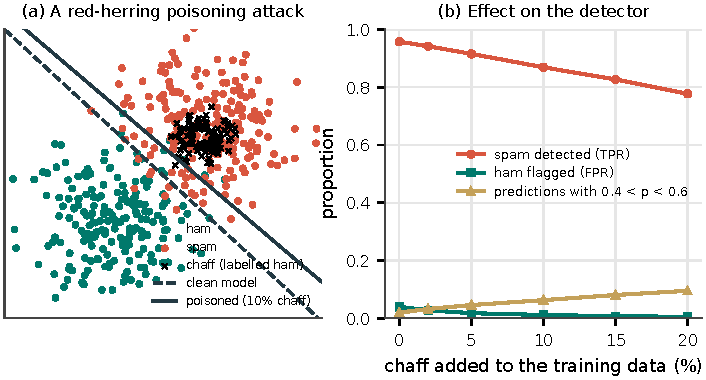
\includegraphics[width=\textwidth]{ch03/poisoning}
\caption{(a) Poisoning moves the decision boundary of a spam detector towards the spam. (b) Detection
rate, false alarm rate and fraction of uncertain predictions as the amount of chaff grows.}
\label{fig:poisoning}
\end{figure}

\paragraph{Attacker knowledge} Knowing the decision function is an important factor: where to place the
chaff, and how much is needed to move the boundary meaningfully, can be hard to determine when the input
is transformed before reaching the classifier (for instance, by a dimensionality reduction). With enough
access, these difficulties can mostly be overcome; the defender's goal is to make such inference
difficult without sacrificing the efficacy of the system.

\paragraph{Defences} There are significant benefits in designing online learning systems that behave
like periodic batch systems: longer periods between retraining give time to inspect the data, a longer
history makes boiling-frog attacks easier to detect, and attackers thrive on short feedback loops.
Poisoning attempts can also be detected by looking for abnormal pockets of traffic (coming from the same
addresses or networks, or sharing unusual characteristics); by keeping a \emph{calibration\index{calibration|textbf} set} of
handcrafted normal and malicious data on which every retrained model is tested; and by monitoring\index{monitoring} the
fraction of predictions that fall near the decision boundary, as in \cref{fig:poisoning}b: a sudden rise
(say, from 30\% to 80\% of the points in the band) suggests that someone is pushing the boundary. There is
no definitive recipe; this is an active area of research, and monitoring is the subject of Unit~6.

\subsection{Evasion attacks}

\emph{Evasion\index{evasion attack|textbf}} is an exploratory attack: the attacker finds adversarial examples\index{adversarial example} that the deployed model
misclassifies, without any influence on its training. Evasion affects every kind of classifier,
traditional and deep, and can have real-world consequences, from road signs to malware detection
\citep{biggio2013evasion}. Perturbations are easy to apply to images, where changing a few pixel
intensities is invisible; applying them to executables is harder, because the modified binary must remain
valid and keep its malicious behaviour, but it has been done.

\begin{pylisting}[label={lst:fgsm}]{FGSM on handwritten digits: white box, transfer and adversarial training}
import numpy as np
from sklearn.datasets import load_digits
from sklearn.ensemble import RandomForestClassifier
from sklearn.linear_model import LogisticRegression
from sklearn.model_selection import train_test_split
from sklearn.neural_network import MLPClassifier

X, y = load_digits(return_X_y=True)
X = X / 16.0                                                    # pixels in [0, 1]
X_tr, X_te, y_tr, y_te = train_test_split(X, y, test_size=0.4, random_state=0, stratify=y)

def fgsm(model, X, y, eps):
    """Fast gradient sign method for a softmax (multinomial logistic) model."""
    P = model.predict_proba(X)
    P[np.arange(len(y)), y] -= 1.0                              # d loss / d logits
    grad = P @ model.coef_                                       # d loss / d input
    return np.clip(X + eps * np.sign(grad), 0, 1)

lr = LogisticRegression(max_iter=3000).fit(X_tr, y_tr)
mlp = MLPClassifier((100,), max_iter=1000, random_state=0).fit(X_tr, y_tr)
rf = RandomForestClassifier(300, random_state=0).fit(X_tr, y_tr)
robust = LogisticRegression(max_iter=3000).fit(np.r_[X_tr, fgsm(lr, X_tr, y_tr, 0.15)],
                                               np.r_[y_tr, y_tr])    # adversarial training
print("eps   LR (white  MLP (trans-  RF (trans-  robust LR:   robust LR:")
print("      box)       ferred)      ferred)     old attack   adaptive")
for eps in (0.0, 0.05, 0.1, 0.2):
    Xa = fgsm(lr, X_te, y_te, eps)                   # crafted on the original LR
    Xr = fgsm(robust, X_te, y_te, eps)               # crafted on the robust LR itself
    print(f"{eps:.2f}  {lr.score(Xa, y_te):.3f}      {mlp.score(Xa, y_te):.3f}        "
          f"{rf.score(Xa, y_te):.3f}       {robust.score(Xa, y_te):.3f}        "
          f"{robust.score(Xr, y_te):.3f}")
\end{pylisting}
\begin{pyoutput}
eps   LR (white  MLP (trans-  RF (trans-  robust LR:   robust LR:
      box)       ferred)      ferred)     old attack   adaptive
0.00  0.972      0.979        0.971       0.940        0.940
0.05  0.873      0.851        0.892       0.940        0.720
0.10  0.641      0.534        0.627       0.926        0.325
0.20  0.090      0.032        0.241       0.871        0.006
\end{pyoutput}

\Cref{lst:fgsm} and \cref{fig:adversarial} attack a logistic regression trained on images of handwritten
digits with the fast gradient sign\index{fast gradient sign method (FGSM)} method of \cref{eq:fgsm}. Changing every pixel by 0.1 (on a 0--1
scale) reduces its accuracy from 0.972 to 0.641, and by 0.2 to 0.090. The same adversarial images,
crafted only with the logistic regression, also fool a neural network (0.534 at $\epsilon=0.1$) and a
random forest (0.627), neither of which the attacker has seen: this is transferability.

\begin{figure}[htbp]
\centering
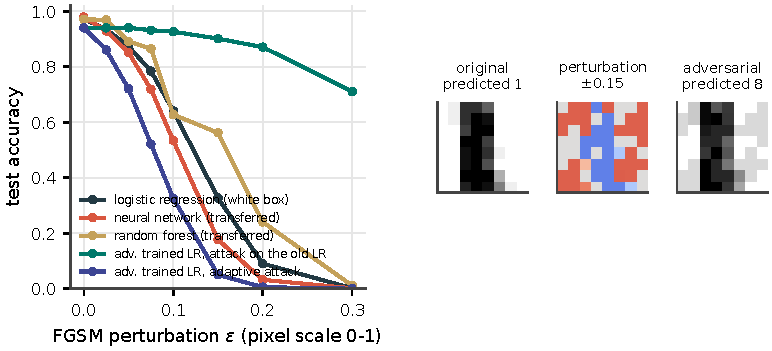
\includegraphics[width=\textwidth]{ch03/adversarial_digits}
\caption{Evasion with the fast gradient sign method on handwritten digits. Left: accuracy as a function
of the size of the perturbation, for the attacked model, two models that receive the transferred
examples, and an adversarially trained model. Right: an image, the perturbation and the adversarial image.}
\label{fig:adversarial}
\end{figure}

\paragraph{Defences} There are no robust general defences against evasion. The general idea is to make it
harder for the attacker to obtain information about the gradients of the decision surface:
\begin{itemize}
  \item \emph{adversarial training\index{adversarial training|textbf}} adds adversarial examples with their correct labels to the training
        data \citep{goodfellow2015explaining}, ideally generating them against the current model at every
        step of training \citep{madry2018towards}. It tries to cover the parts of the input space that the
        training data do not reach, which can never be done exhaustively. In \cref{lst:fgsm}, a model
        trained once with adversarial images is robust to the attack it was trained on (0.871 at
        $\epsilon=0.2$), but an attacker who crafts new examples against \emph{it} breaks it completely
        (0.006): the defence only raised the bar for an attacker who does not adapt;
  \item \emph{defensive distillation\index{model distillation|textbf}} \citep{papernot2016distillation} trains a second model on the
        probability outputs of the first (the distillation of \cref{sec:drawbacks}), which smooths the
        decision surface and hides useful gradients; stronger attacks were soon shown to defeat it
        \citep{carlini2017towards}. More generally, defences that merely mask the gradients give a false
        sense of security \citep{athalye2018obfuscated}.
\end{itemize}
Many practical defences fail against adaptive attacks, so robustness must be evaluated under an explicit threat
model\index{threat model} and attack budget. A defence may raise the cost of attacks or provide guarantees within stated constraints;
neither establishes security against every possible adversary.

\begin{example}{A good-word attack on a spam filter}{goodword}
A spammer cannot see the filter but can test messages against it. \citet{lowd2005good} showed that adding
a few ``good'' words, typical of legitimate e-mail, is enough to get much spam through statistical filters.
\Cref{lst:goodword} simulates the attack on a logistic regression filter over a vocabulary of 60 words:
the attacker greedily adds the word that most lowers the spam probability, one query per candidate word.
Three added words let 36\% of the detected spam through, five words 67\%, and ten words 98\%. Retraining the
filter with attacked spam labelled as spam makes the attack harder (23\%, 55\% and 95\%) without stopping
it (\cref{fig:evasion}).
\end{example}

\begin{pylisting}[label={lst:goodword}]{A black-box good-word attack and adversarial training}
import numpy as np
from sklearn.linear_model import LogisticRegression

def emails(n, seed):
    """Bag of words: words 0-14 are 'spammy', 15-29 'hammy' and 30-59 neutral."""
    rng = np.random.default_rng(seed)
    spam = np.r_[np.ones(n // 2, int), np.zeros(n - n // 2, int)]
    p = np.where(spam[:, None] == 1, [0.30] * 15 + [0.05] * 15 + [0.1] * 30,
                 [0.03] * 15 + [0.25] * 15 + [0.1] * 30)
    return (rng.random((n, 60)) < p).astype(float), spam

def good_word_attack(model, x, budget=10):
    """Add, one at a time, the word that most lowers P(spam) (one query per candidate)."""
    x = x.copy()
    for k in range(budget + 1):
        if model.predict_proba(x[None])[0, 1] < 0.5:
            return k, x
        if k == budget:
            return None, x
        cand = np.flatnonzero(x == 0)
        Z = np.repeat(x[None], len(cand), axis=0)
        Z[np.arange(len(cand)), cand] = 1
        x[cand[np.argmin(model.predict_proba(Z)[:, 1])]] = 1

X, y = emails(4000, 0)
X_test, y_test = emails(2000, 1)
clf = LogisticRegression(max_iter=2000).fit(X, y)
adv = np.array([good_word_attack(clf, x)[1] for x in X[y == 1][:600]])
X_aug, y_aug = np.r_[X, adv], np.r_[y, np.ones(len(adv), int)]     # attacked spam is spam
robust = LogisticRegression(max_iter=2000).fit(X_aug, y_aug)
for name, m in [("standard filter", clf), ("adversarially trained", robust)]:
    caught = X_test[(y_test == 1) & (m.predict(X_test) == 1)][:300]
    need = [good_word_attack(m, x)[0] for x in caught]
    rates = [np.mean([k is not None and k <= b for k in need]) for b in (1, 3, 5, 10)]
    det = m.predict(X_test)[y_test == 1].mean()
    print(f"{name:22s} detection={det:.3f}  evasion with 1/3/5/10 words: "
          + " ".join(f"{r:.2f}" for r in rates))
\end{pylisting}
\begin{pyoutput}
standard filter        detection=0.974  evasion with 1/3/5/10 words: 0.06 0.36 0.67 0.98
adversarially trained  detection=0.974  evasion with 1/3/5/10 words: 0.04 0.23 0.55 0.95
\end{pyoutput}

\begin{figure}[htbp]
\centering
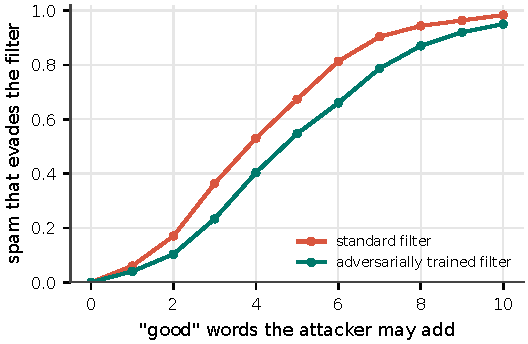
\includegraphics[width=0.66\textwidth]{ch03/evasion}
\caption{Fraction of detected spam that evades the filter as a function of the number of good words the
attacker may add, for a standard and an adversarially trained filter.}
\label{fig:evasion}
\end{figure}

\subsection{Other threats}

Poisoning\index{poisoning attack} and evasion\index{evasion attack} are not the only threats. A model offered through an API\index{API} can be \emph{stolen} by
querying it and training a copy \citep{tramer2016stealing}; \emph{membership inference} attacks find out
whether a given record was part of the training data, a privacy breach for medical or financial data
\citep{shokri2017membership}; \emph{backdoors\index{backdoor criterion|textbf}} hidden in training data or in pre-trained models make a
model misbehave only when a secret trigger is present \citep{gu2017badnets}; and applications built on
large language models\index{large language model (LLM)}\index{language model} can be hijacked by instructions hidden in the content they process, a \emph{prompt\index{prompt|textbf}
injection\index{prompt injection|textbf}} \citep{greshake2023not}.

\begin{keyidea}
Being secure and robust is a prerequisite for deploying machine learning, but the difficulty of avoiding
attacks is not a reason to shy away from it. Machine learning can behave in unexpected ways in adversarial
environments; this is not a ``failure'' of machine learning but a sign of improperly calibrated
expectations. Knowing the types of vulnerability helps to make fewer false assumptions about what a model
can do.
\end{keyidea}

% ---------------------------------------------------------------------

% =====================================================================
\section{Regulation: the European AI Act}\label{sec:aiact}

Much of what this unit has presented as good practice is now law in the European Union. Regulation (EU)
2024/1689, the \emph{AI Act\index{AI Act|textbf}}, entered into force on 1 August 2024 as the first comprehensive law on artificial
intelligence \citep{eu2024aiact}. It does not regulate techniques but \emph{uses}: the same classifier may be
unregulated when it filters spam and heavily regulated when it decides who gets a loan. It complements earlier
rules, such as the General Data Protection Regulation\index{GDPR}, which already gives people the right not to be subject
to decisions based solely on automated processing that significantly affect them, with safeguards such as
human intervention\index{intervention} \citep{gdpr2016,wachter2017right}. For decisions based on the output of the high-risk\index{AI Act!high-risk systems} systems of Annex~III\index{AI Act!Annex III}
(except those of its point~2, critical infrastructure) that produce legal effects, or similarly significantly affect a
person in a way that they consider adverse to their health, safety or fundamental rights, the AI Act adds a right to
obtain clear and meaningful explanations of the role of the system in the decision procedure and of the main elements
of the decision (Article~86\index{AI Act!Article 86}), subject to the exceptions and restrictions of other laws. It is not a general obligation
to produce actionable or counterfactual explanations\index{counterfactual explanation} for every decision.

\subsection{A risk-based approach}

The AI Act\index{AI Act} sorts AI systems into four levels of risk:
\begin{itemize}
  \item \emph{unacceptable risk}: practices that are prohibited, such as manipulating people by exploiting
        their vulnerabilities, social scoring, predicting that a person will commit a crime solely from their
        profile, building facial recognition databases by untargeted scraping of images, recognising emotions in
        workplaces and schools, inferring sensitive attributes\index{protected attribute} such as religion or sexual orientation from
        biometric data, and, with narrow exceptions, real-time remote biometric identification in public spaces
        for law enforcement;
  \item \emph{high risk\index{AI Act!high-risk systems|textbf}}: systems that are safety components of products already regulated in the EU (medical
        devices, machinery, toys) and systems used in the areas listed in Annex~III\index{AI Act!Annex III} of the Act: biometrics,
        critical infrastructure, education (admission, assessment), employment (recruitment, promotion,
        monitoring of workers), access to essential services (eligibility for public benefits, the
        creditworthiness and credit scoring of people, risk assessment and pricing in life and health insurance,
        triage of emergency calls), law enforcement, migration and border control, and the administration of
        justice and democratic processes;
  \item \emph{limited risk}: systems subject to transparency obligations: people must be told when they are
        interacting with a chatbot, and content generated or manipulated by AI, such as deepfakes, must be
        labelled as such;
  \item \emph{minimal risk}: everything else, such as spam filters or film recommenders\index{recommender system}, with no specific
        obligations beyond the duty to take measures that support the \emph{AI literacy\index{AI literacy|textbf}} of the staff who use
        AI (as amended in 2026, Article~4 does not require guaranteeing a specific individual level).
\end{itemize}
\emph{General-purpose AI models}, such as large language models\index{large language model (LLM)}, have their own obligations: technical documentation,
information for the providers that build systems on them, a policy to respect copyright and a summary of the
content used for training; the most capable ones, presumed to pose systemic risks, must also be evaluated, including
adversarial testing, have their serious incidents reported, and be adequately protected.

\subsection{Obligations for high-risk systems}

The \emph{providers} of high-risk\index{AI Act!high-risk systems} systems, those who develop them or place them on the market, must meet a set of
requirements before and after the system is deployed. Read with the eyes of a data scientist, they are a summary of this
book (\cref{tab:aiact}). The \emph{deployers}, the organisations that use the systems, must use them according to their
instructions, assign human oversight to competent people, make sure that the input data are relevant, monitor their
operation and keep their logs; public bodies, and those that use AI for credit scoring or to price life and health
insurance, must also assess the impact of the system on fundamental rights before using it.

\begin{table}[htbp]
\centering\small
\caption{Requirements of the AI Act for high-risk systems, and where this book deals with them.}\label{tab:aiact}
\begin{tabularx}{\textwidth}{@{}>{\raggedright\arraybackslash}p{3.0cm}>{\raggedright\arraybackslash}X>{\raggedright\arraybackslash}p{3.1cm}@{}}
\toprule
Requirement & What it asks for & In this book\\
\midrule
Risk management (Art.~9) & identify, estimate and mitigate the risks of the system throughout its life cycle & Units
\ref{ch:evaluation}, \ref{ch:reliable} and \ref{ch:monitoring}\\
Data governance (Art.~10) & relevant and representative training, validation and test data, examined for possible
biases & \cref{sec:protocols,sec:fairness,sec:shift}\\
Documentation and logs (Arts.~11--12) & technical documentation of the system, and automatic recording of its operation
& model cards \citep{mitchell2019model}; \cref{sec:infrastructure}\\
Transparency (Art.~13) & instructions that let deployers understand the system and use its outputs appropriately &
\cref{sec:interpretability}\\
Human oversight (Art.~14) & people able to understand, monitor, override and stop the system, aware of the tendency to
over-rely on it & \cref{sec:cautious}; \cref{sec:interpretability}\\
Accuracy, robustness, cybersecurity (Art.~15) & declared levels of accuracy, resilience to errors and to attacks such as
poisoning and adversarial examples & \cref{ch:evaluation}; \cref{sec:adversarial}\\
Quality management and conformity (Arts.~17, 43) & documented processes, and an assessment of conformity before the system
is placed on the market & \cref{sec:infrastructure}\\
Post-market monitoring (Arts.~72--73) & collect and analyse data on the performance of the system in use, and report
serious incidents & \cref{ch:monitoring}\\
\bottomrule
\end{tabularx}
\end{table}

\subsection{Timeline and enforcement}

The obligations apply in stages. The prohibitions and the duty to support AI literacy\index{AI literacy} apply since 2 February 2025, and the
obligations for general-purpose models since 2 August 2025. The obligations for high-risk\index{AI Act!high-risk systems} systems were due to apply from
August 2026, but an amendment adopted in 2026, the \emph{Digital Omnibus\index{Digital Omnibus on AI|textbf} on AI} (Regulation (EU) 2026/1744, in force since 27 July 2026),
postponed them to fixed dates: those for the systems of Annex~III\index{AI Act!Annex III}, such as credit scoring, apply from 2 December 2027, and those for systems
embedded in regulated products from 2 August 2028 \citep{eu2026omnibus}. The amendment also widened the possibility of
processing personal data when strictly necessary to detect and correct biases, which matters because, as we saw in
\cref{sec:fairness}, measuring discrimination usually requires the very attributes that one would like to leave out. Fines
reach 35 million euros or 7\% of a company's worldwide annual turnover for prohibited practices, and 15 million euros or 3\% for
other infringements. Each member state designates authorities to supervise the market; Spain created the first national
agency, the Spanish Agency for the Supervision of Artificial Intelligence (AESIA), while the European Commission's AI Office
supervises general-purpose models. This section describes the AI Act\index{AI Act} as amended in 2026, as checked on 12 October 2026;
its obligations and dates must be rechecked for each edition.

\subsection{A credit-scoring model under the AI Act}

Consider the credit model of \cref{sec:fairness} in a European bank. It is a high-risk\index{AI Act!high-risk systems} system, so before using it the bank, as
its provider, must document its data and their representativeness, its performance overall and for the relevant groups of
applicants (\cref{lst:credit}), its known limitations and the conditions under which it should not be used. Its decisions must be
logged, and a person must be able to review and override them: the cautious classifiers\index{cautious classifier} of \cref{sec:cautious}, which
delegate\index{delegation} uncertain cases to an analyst, are a natural design. Rejected applicants may have the right to a clear and meaningful
explanation of the role of the system in the decision (Article~86\index{AI Act!Article 86}); offering an explanation they can act on, such as the
counterfactual explanations\index{counterfactual explanation} of \cref{sec:examplebased} (``with a debt ratio below 35\%, the loan would have been approved''),
is a design choice that goes beyond that right. Once in use, the model must be monitored for drift and for changes in its performance across groups, and serious
incidents must be reported (\cref{ch:monitoring}). None of these obligations requires a new technique; all of them require using the
techniques of this book systematically, and documenting that they were used. The techniques help to meet the
obligations, but they do not replace conformity assessment, legal documentation and the procedures the law requires.

\begin{keyidea}
The AI Act\index{AI Act} regulates what a system is used for, not how it is built. For high-risk uses it turns evaluation, data governance,
documentation, human oversight, robustness and monitoring from good practice into legal obligations.
\end{keyidea}

% =====================================================================
\section{Summary}\label{sec:summary3}

\begin{itemize}
  \item Unfairness can enter a machine learning system at every stage: measurement, learning, action and
        feedback. Removing the sensitive attribute\index{protected attribute} does not remove it.
  \item The main group fairness\index{fairness} criteria (independence, separation\index{fairness!separation} and sufficiency\index{fairness!sufficiency}) are conditional
        independences that are generally incompatible; choosing one is choosing whose errors matter. They
        are diagnostics, not certificates, and they cannot distinguish mechanisms with the same
        observational distribution.
  \item Causal models distinguish observing from intervening. Confounders\index{confounder} must be adjusted for, mediators\index{mediator}
        and colliders\index{collider} must not; counterfactuals answer questions about alternatives to what happened. Both
        are needed to reason about discrimination.
  \item Interpretability is needed because objectives are never completely specified. Interpretable models
        (linear, logistic, trees, rules) can be read directly, with care about their assumptions.
  \item Model-agnostic methods (PDP, ICE\index{individual conditional expectation}, interaction strength, permutation importance\index{feature importance!permutation}, surrogates\index{global surrogate}, LIME\index{LIME} and
        Shapley\index{Shapley values} values) explain any model, but each answers a different question and has limitations that
        must be known.
  \item Example-based explanations (counterfactuals, prototypes\index{prototypes and criticisms} and criticisms, influential instances\index{influential instance})
        explain with instances; adversarial examples\index{adversarial example} are counterfactuals designed to deceive.
  \item Machine learning systems can be attacked during training (poisoning\index{poisoning attack}) and deployment (evasion\index{evasion attack});
        adversarial examples transfer between models, and defences raise the cost of attacks without
        eliminating them.
  \item The European AI Act\index{AI Act} regulates uses by their risk: it prohibits some practices and, for high-risk\index{AI Act!high-risk systems} systems such as
        credit scoring, requires risk management, data governance, documentation, logging, transparency, human oversight,
        accuracy, robustness and monitoring after deployment.
\end{itemize}

\section*{Bibliographic notes}
\phantomsection\addcontentsline{toc}{section}{Bibliographic notes}

The fairness\index{fairness} and causality\index{causality} sections follow the approach of \citet{barocas2023fairness}, whose book is the
best introduction to the field; \citet{mehrabi2021survey} survey the sources of bias and the mitigation
techniques. \citet{pearl2018book} is an accessible introduction to causal reasoning, and
\citet{pearl2009causality}, \citet{peters2017elements} and \citet{hernan2020causal} are more technical
references. The interpretability sections follow \citet{molnar2022interpretable}, which describes many more
methods; \citet{miller2019explanation} reviews what the social sciences say about explanations and
\citet{doshivelez2017towards} discuss how to evaluate interpretability. \citet{chio2018machine} cover machine
learning for security, and \citet{biggio2018wild} review ten years of adversarial machine learning\index{adversarial machine learning}.

\section*{Exercises}
\phantomsection\addcontentsline{toc}{section}{Exercises}

\begin{enumerate}[label=\textbf{3.\arabic*},ref=3.\arabic*,leftmargin=*,itemsep=6pt]
  \item\label{exr3:groups} A hiring model is applied to 600 candidates of group $a$ (400 qualified) and 400
        of group $b$ (160 qualified). It selects 300 qualified and 40 unqualified candidates of group $a$,
        and 96 qualified and 24 unqualified of group $b$. Compute, for each group, the selection rate, the
        true and false positive rates\index{false positive rate} and the positive predictive value\index{predictive value!positive}. Does the model pass the
        four-fifths rule? Which criteria hold?
  \item\label{exr3:chouldechova} Two groups have prevalences\index{prevalence} 0.6 and 0.3. A classifier has $\PPV=0.8$ and
        $\TPR=0.7$ in both groups. Use \cref{eq:chouldechova} to compute the false positive rate of each
        group.
  \item\label{exr3:simpson} Department X admits 80 of 100 men and 18 of 20 women; department Y admits 4 of
        20 men and 30 of 100 women. Compute the aggregate admission rates and the rates adjusted with the
        overall distribution of applicants across departments.
  \item\label{exr3:heart} In the heart disease model of \cref{ex:heart}, change the probabilities to
        $P(U_1=1)=0.4$, $P(U_2=1)=0.5$ and $P(U_3=1)=0.25$. Compute $P(H=1)$, $P(H=1\mid W=1)$ and
        $P(H=1\mid\mathrm{do}(W:=1))$.
  \item\label{exr3:adjust} In a causal graph\index{causal graph}, age $Z$ influences both a treatment $X$ and an outcome $Y$; the
        treatment acts on $Y$ directly and through a biomarker $M$; and both $X$ and $Y$ influence whether a
        patient attends a follow-up visit $C$. To estimate the total effect of $X$ on $Y$, which variables
        should you adjust for?
  \item\label{exr3:traffic} Repeat \cref{ex:traffic} with a probability of a bad day $P(U=1)=0.3$ (accidents
        still have probability 0.5). Compute the interventional probability $P\{Y=0\mid\mathrm{do}(X:=0)\}$
        and the counterfactual probability that route 0 would have been fast, given that route 1 was
        slow.
  \item\label{exr3:odds} A logistic regression has a weight of 0.4 for the number of years of education.
        What is the odds ratio\index{odds ratio}? If an applicant has a probability of 0.5, what is their probability with one
        more year of education?
  \item\label{exr3:adjr2} A linear model with 10 features has $R^2=0.30$ on 100 examples. Compute the
        adjusted $R^2$.
  \item\label{exr3:pdp} A model is $f(x_1,x_2)=x_1x_2$, and $x_2$ takes the values $-1$ and $1$ with equal
        probability, independently of $x_1$, which has mean zero and positive variance. Draw the PDP of $x_1$ and its ICE\index{individual conditional expectation} curves. What do you
        conclude?
  \item\label{exr3:shapley} The model $f(x_1,x_2)=2x_1+3x_2+x_1x_2$ has independent features with mean 0.
        Compute the Shapley\index{Shapley values} values of the instance $(1,1)$ and check the efficiency property.
  \item\label{exr3:cf} A bank accepts applicants with $s(x)=0.5\,\text{income}-10\,\text{debt}-2\geq0$
        (income in thousand euros). An applicant has an income of 30 and a debt ratio of 1.5. What is the
        smallest change of income alone, and of debt alone, that gets the loan? If the median absolute
        deviations are 8 and 0.5, which counterfactual does the method of Wachter et al.\ prefer?
  \item\label{exr3:fgsm} A linear classifier has logit $z=w^\top x+b$ with 64 inputs, all with weights of
        absolute value 0.5. By how much can an FGSM\index{fast gradient sign method (FGSM)} perturbation with $\epsilon=0.05$ change the logit? What
        does this tell you about high-dimensional inputs?
  \item\label{exr3:taxonomy} Classify each attack according to \cref{tab:attacks}: (a) a fraudster sends
        many crafted transactions to a fraud model that is retrained daily, so that it learns to accept
        one particular kind of fraud; (b) a spammer rewrites messages until they get through a fixed
        filter; (c) an attacker floods a self-updating intrusion detector with noise until operators
        disable it because of the false alarms.
  \item\label{exr3:monitor} A spam detector usually has 30\% of its predictions in the band
        $0.4<p<0.6$. During the last week the figure rose to 80\%. List possible explanations and the
        actions you would take.
  \item\label{exr3:aiacttiers} Classify each system by its level of risk under the AI Act\index{AI Act}: (a) software that ranks the CVs of
        candidates for a job; (b) a spam filter; (c) a chatbot that answers customers' questions; (d) a system that scores the
        trustworthiness of citizens from their social behaviour, for a public authority; (e) a model that decides the credit
        limit of a credit card; (f) a system that recognises the emotions of the employees of a call centre.
  \item\label{exr3:aiactplan} For the credit model of \cref{sec:fairness}, describe the evidence a bank should prepare for
        Articles 10, 13, 14 and 72 of the AI Act (\cref{tab:aiact}), naming a technique of this book for each.
\end{enumerate}

\section*{Solutions to selected exercises}
\phantomsection\addcontentsline{toc}{section}{Solutions to selected exercises}

\begin{description}[font=\bfseries,leftmargin=0pt,itemsep=5pt]
  \item[\ref{exr3:groups}] Group $a$: selection $340/600=0.57$, $\TPR=300/400=0.75$, $\FPR=40/200=0.20$,
        $\PPV=300/340=0.88$. Group $b$: selection $120/400=0.30$, $\TPR=96/160=0.60$, $\FPR=24/240=0.10$,
        $\PPV=96/120=0.80$. The ratio of selection rates is $0.30/0.57=0.53<0.8$: the model fails the
        four-fifths rule. None of the criteria holds exactly.
  \item[\ref{exr3:chouldechova}] $\FPR=\frac{0.6}{0.4}\cdot\frac{0.2}{0.8}\cdot0.7=0.26$ and
        $\frac{0.3}{0.7}\cdot\frac{0.2}{0.8}\cdot0.7=0.075$: equal $\PPV$ and $\TPR$ force very different
        false positive rates\index{false positive rate}.
  \item[\ref{exr3:simpson}] Aggregate: men $84/120=0.70$, women $48/120=0.40$. Each department receives half
        of the 240 applicants, so the adjusted rates are $0.5\cdot0.8+0.5\cdot0.2=0.50$ for men and
        $0.5\cdot0.9+0.5\cdot0.3=0.60$ for women: women are favoured in both departments.
  \item[\ref{exr3:heart}] $P(H=1)=0.6\cdot0.25=0.15$; $P(H=1\mid W=1)=0.25$, since overweight implies no
        exercise; $P(H=1\mid\mathrm{do}(W:=1))=0.15$, unchanged.
  \item[\ref{exr3:adjust}] Adjust for age $Z$ (a confounder\index{confounder}). Do not adjust for the biomarker $M$ (a mediator\index{mediator}:
        it would remove part of the effect) nor for the follow-up visit $C$ (a collider\index{collider}: it would create a
        spurious association).
  \item[\ref{exr3:traffic}] $P\{Y=0\mid\mathrm{do}(X:=0)\}=0.7\cdot0.5=0.35$. The evidence has probability
        $1-0.7\cdot0.5=0.65$ and $P(U=0\mid E)=0.7\cdot0.5/0.65=0.54$, so the counterfactual probability is
        $0.54\cdot0.5=0.27$.
  \item[\ref{exr3:odds}] $e^{0.4}=1.49$; the odds go from 1 to 1.49, so the probability becomes
        $1.49/2.49=0.60$.
  \item[\ref{exr3:adjr2}] $\bar R^2=1-0.7\cdot99/89=0.22$.
  \item[\ref{exr3:pdp}] The PDP is $x_1\E[x_2]=0$, a flat line, while the ICE\index{individual conditional expectation} curves are lines of slope $+1$
        and $-1$: the feature matters a lot, but its effect is pure interaction ($H^2=1$, which needs $\E[x_1]=0$: with mean $m$ and variance $v$
        it would be $v/(v+m^2)$), and the PDP hides it.
  \item[\ref{exr3:shapley}] $v(\emptyset)=0$, $v(\{1\})=2$, $v(\{2\})=3$, $v(\{1,2\})=6$. Then
        $\phi_1=\frac12[(2-0)+(6-3)]=2.5$ and $\phi_2=\frac12[(3-0)+(6-2)]=3.5$, which add up to
        $6=f(1,1)-\E[f]$: the interaction term is split equally.
  \item[\ref{exr3:cf}] $s(x)=15-15-2=-2$. Income alone: $+4$ thousand euros; debt alone: $-0.2$. Costs in MAD
        units: $4/8=0.5$ and $0.2/0.5=0.4$, so the method prefers reducing the debt ratio to 1.3.
  \item[\ref{exr3:fgsm}] Each input moves by 0.05 in the direction of its weight, so the logit changes by
        $\epsilon\|w\|_1=0.05\cdot64\cdot0.5=1.6$. Tiny changes in many inputs add up: the more dimensions, the
        larger the effect of an imperceptible perturbation.
  \item[\ref{exr3:taxonomy}] (a) Causative, targeted, integrity. (b) Exploratory, targeted (the spammer
        wants ``legitimate''), integrity. (c) Causative, indiscriminate, availability.
  \item[\ref{exr3:monitor}] A poisoning\index{poisoning attack} attempt that pushes the boundary, a genuine change in the data
        (drift), or a change in an upstream feature pipeline. Stop automatic retraining, compare the recent
        training data with the history (sources, addresses, feature distributions), test the current model
        on the calibration set, and roll back to the last validated model if needed.
  \item[\ref{exr3:aiacttiers}] (a) High risk\index{AI Act!high-risk systems} (employment). (b) Minimal risk. (c) Limited risk: users must be told that they are
        talking to a machine. (d) Prohibited (social scoring). (e) High risk (creditworthiness of people). (f) Prohibited:
        emotion recognition in the workplace, except for medical or safety reasons.
  \item[\ref{exr3:aiactplan}] Article 10: the representativeness of the training data and an analysis of bias, such as the
        fairness\index{fairness} criteria of \cref{sec:fairness}. Article 13: documentation of the model and of how to read its outputs, with
        explanations (\cref{sec:interpretability}). Article 14: a procedure for analysts to review and override decisions, for
        instance with a cautious classifier\index{cautious classifier} that delegates\index{delegation} uncertain cases (\cref{sec:cautious}). Article 72: a monitoring plan
        for drift and for performance by group (\cref{ch:monitoring}).
\end{description}

